% !TeX root = ../../Book3.tex
% 纲要标题：## 附录 D　局部环、幂级数与结构定理
% 纲要位置：工作记录/计划纲要.md:2944

\chapter{局部环、幂级数与结构定理}
\label{b3:app:D}
\BookChapterNumber{b3:app:D}

\begin{chapterabstract}
局部化、Hensel 化、完备化与收敛幂级数提供了研究局部方程的不同环境。本附录先用实际环同态比较它们，再说明 Cohen 结构定理如何把完备局部环表示为幂级数环的商。形式与收敛 Weierstrass 除法分别由理想阶数与范数估计得到有限余式，尖点与节点的计算展示分支、切锥及交数的差别。最后引入形式纤维与卓越性，并准确区分 Artin 逼近、收敛性和代数化。
\end{chapterabstract}

\begin{learninggoals}
\begin{itemize}
\item 说明 Hensel 化与完备化各自的泛性质，辨认代数、收敛和形式级数之间的包含。
\item 说明系数对象存在性所用的定理，并在选定系数对象后证明幂级数商表示。
\item 证明形式与收敛 Weierstrass 除法和预备定理，并用余式写出相应商模的有限生成元。
\item 对曲线计算分支、切锥、局部交数及权初始部分，不把这些量互相替代。
\item 写出卓越性的三个条件，并说明有限阶逼近中给定精度、形式解和准确解的量词次序。
\end{itemize}
\end{learninggoals}

复系数的形式级数 \(\sum_{n\ge0}n!x^n\) 在 \(\mathbb C[[x]]\) 中完全合法，因为任意固定次数的系数只由有限步运算决定；但它在任意 \(x\ne0\) 处都不收敛。相同的“幂级数”记号因而可能指两种不同对象：形式局部环中的元素，或某个邻域上的解析函数芽。证明前者的除法公式，不能自动宣称后者也有收敛的商与余式。

\ProseParagraphBreak

从局部环出发，可以先完备化以记录所有相容的有限阶近似；若只想提升可分根而不添入所有形式极限，则还有 Hensel 化。Cohen 结构、Weierstrass 除法\footnote{魏尔斯特拉斯（Karl Theodor Wilhelm Weierstrass，1815-1897），德国数学家，推动分析学的严格化，并在复变函数与幂级数理论中作出重要贡献。}和曲线的局部计算分别告诉我们这些环境能够表示哪些方程。比较它们的同态及适用条件，才能在形式解、收敛解和代数解之间作出可靠区分。

\ProseParagraphBreak

本附录需要\chapref{b3:ch:13}的完备化、\chapref{b3:ch:18}的正则局部环和\chapref{b3:ch:19}的完全交；Hensel 性及 Hensel 化采用\chapref{b3:ch:23}的定义与存在性结论。收敛部分只在复系数下讨论，另需多复变量幂级数、函数芽和恒等定理的初步知识。形式部分不依赖解析收敛。

\ProseParagraphBreak
幂级数商的具体构造、形式与收敛 Weierstrass 除法、解析环的基本性质、有限自由模结论及曲线算例均给出证明。系数域及 Cohen 系数环的存在、代数幂级数收敛、卓越环的基本性质与 Artin 逼近给出证明概要，并注明省略的技术引理及出处。标准基的主要讲授位置在\appref{b3:app:F}，本附录只说明它与局部结构的联系。

\ProseParagraphBreak
\cref{b3:fig:D-local-environments}把两种比较放在一起。一般 Noether 局部环 \((A,\mathfrak m)\) 的 Hensel 化与完备化通过自然局部同态相连；复坐标情形还可以按代数方程和收敛条件区分三种级数环。图中的箭头不表示这些环相同。

\begin{figure}[htbp]
\centering
\[
\begin{tikzcd}[column sep=8em]
A \arrow[r,"\text{自然局部同态}"] & A^{\mathrm h} \arrow[r,"\text{自然局部同态}"] & \widehat A
\end{tikzcd}
\]
Hensel 化 \(A^{\mathrm h}\) 满足向 Hensel 局部环分解的泛性质；\(\widehat A=\varprojlim_n A/\mathfrak m^n\) 则是原环的理想进完备化。
\[
\begin{tikzcd}[column sep=large]
\mathbb C[x]_{(x)} \arrow[r,hook] & \mathbb C\langle x\rangle \arrow[r,hook] & \mathbb C\{x\} \arrow[r,hook] & \mathbb C[\![x]\!]
\end{tikzcd}
\]
\caption{局部环与幂级数环境的比较}
\label{b3:fig:D-local-environments}
\end{figure}

这里 \(x=(x_1,\ldots,x_n)\)，\(n\ge1\)。代数级数满足有理函数域上的代数方程，收敛级数具有正的收敛半径，形式级数则只要求各项系数给定。具体映射及 Hensel 化与代数级数的关系见\secref{b3:sec:D01}。

\ProseParagraphBreak
Cohen 结构可读松村英之\cite[Theorem 28.3, pp. 215--216; Theorems 29.1--29.4, pp. 223--226]{Matsumura1989CommutativeRingTheory}；收敛幂级数与 Weierstrass 方法见永田雅宜\cite[\S45, (45.1), (45.3), (45.5)--(45.6), pp. 190--194]{Nagata1975LocalRings}。卓越性采用松村英之\cite[\S32, pp. 259--260]{Matsumura1989CommutativeRingTheory}的三个条件；逼近讨论 Artin\cite[Theorem (1.10), p. 26; Section 5, pp. 42--50]{Artin1969AlgebraicApproximation}中的代数情形及其 Jacobian 修正方法。

% !TeX root = ../../Book3.tex
% 纲要标题：### D.1 局部环与幂级数环的比较
% 纲要位置：工作记录/计划纲要.md:2900

\section{局部环与幂级数环的比较}
\label{b3:sec:D01}

相同的有限阶展开可以来自不同的环，允许的无限过程也随之不同。比较局部方程时，应先确定所用环及其间的同态，再问形式解、代数解或收敛解能否互相转换。

% 纲要内容（仅作写作计划，尚非教材正文）：
% * 代数局部环、Hensel 局部环、完备局部环与复收敛幂级数环
% * Hensel 化和完备化的泛性质不同；Hensel 性不意味着完备
% * 代数幂级数与 Hensel 化的识别；解析环基本性质及代数级数收敛的证明在D.3除法之后给出
% * 用实际环同态而不是只凭“函数芽”的直觉说明包含与比较关系
% #### D.1.1 代数、Hensel、完备与解析局部环
% #### D.1.2 Hensel 化与完备化的泛性质
% #### D.1.3 代数、形式与收敛幂级数
% #### D.1.4 局部对象间的环同态与比较关系


\subsection{代数、Hensel、完备与解析局部环}
\label{b3:subsec:D01:01}

\begin{definition}\label{b3:def:algebraic-analytic-local-model}
设 \(k\) 为域，\(n\ge1\)，\(I\subseteq k[x_1,\ldots,x_n]\) 为理想，\(\mathfrak p\) 为商环 \(k[x_1,\ldots,x_n]/I\) 的素理想。有限型 \(k\)-代数在 \(\mathfrak p\) 处的局部化
\[
A=(k[x_1,\ldots,x_n]/I)_{\mathfrak p}
\]
称为一个代数局部环。对 \(k=\mathbb C\)，记
\[
\mathbb C\{x_1,\ldots,x_n\}
=\left\{\sum_\alpha c_\alpha x^\alpha:
c_\alpha\in\mathbb C,\quad
\text{存在 }r>0\text{ 使 }\sum_\alpha|c_\alpha|r^{|\alpha|}<\infty\right\}.
\]
称它为\term[convergentpowerseriesring]{收敛幂级数环}[convergent power series ring]；它的有限生成真理想的商称为这里所讨论的解析局部环。
\end{definition}

收敛级数的和、积仍在一个较小的多圆盘上绝对收敛，因此上述集合是环。常数项非零的级数在原点附近不为零，其倒数仍有收敛展开；常数项为零者不能可逆。故 \(\mathbb C\{x\}\) 是局部环，极大理想为 \((x_1,\ldots,x_n)\)，剩余域为 \(\mathbb C\)。它描述的是原点处的全纯函数芽，而不是在一个预先固定的大区域上都收敛的函数。

\ProseParagraphBreak
形式幂级数环 \(k[\![x_1,\ldots,x_n]\!]\) 不要求系数满足任何大小限制。它的完备性是 \((x_1,\ldots,x_n)\)-进完备性，表达每个次数的系数最终确定；这与复变量函数在某个圆盘内收敛是不同的要求。

\begin{theorem}[收敛幂级数环的基本性质]\label{b3:thm:convergent-series-local-properties}
设 \(n\ge1\)，\(R=\mathbb C\{x_1,\ldots,x_n\}\)，\(\mathfrak m=(x_1,\ldots,x_n)R\)。则 \((R,\mathfrak m)\) 是维数 \(n\) 的 Noether 正则 Hensel 局部环，剩余域为 \(\mathbb C\)，其 \(\mathfrak m\)-进完备化为
\(\mathbb C[\![x_1,\ldots,x_n]\!]\)。
\end{theorem}

证明见\cref{b3:cor:analytic-series-local-properties}，位于\subsecref{b3:subsec:D03:01}的收敛 Weierstrass 除法定理之后。

\subsection{Hensel 化与完备化的泛性质}
\label{b3:subsec:D01:02}

第23章已经定义 Hensel 环并证明完备局部环具有 Hensel 性。其存在性定理给出一个局部同态
\(A\to A^{\mathrm h}\)，使任何从 \(A\) 到 Hensel 局部环的局部同态都唯一经过 \(A^{\mathrm h}\)。这里要求延拓的是代数方程的单根或互素因式；没有要求补入所有相容的极限。

\begin{proposition}\label{b3:prop:completion-continuous-universal}
设 \((A,\mathfrak m)\) 为局部环，\((B,\mathfrak n)\) 为 \(\mathfrak n\)-进完备分离的局部环。每个局部同态 \(u:A\to B\) 唯一延拓为一个连续同态
\(\widehat u:\widehat A\to B\)，其中 \(\widehat A=\varprojlim A/\mathfrak m^r\) 采用逆极限拓扑，\(B\) 采用 \(\mathfrak n\)-进拓扑。
\end{proposition}
\begin{proof}
局部性给出 \(u(\mathfrak m^r)\subseteq\mathfrak n^r\)，因而得到相容的同态
\(A/\mathfrak m^r\to B/\mathfrak n^r\)。取逆极限，并利用 \(B\simeq\varprojlim B/\mathfrak n^r\)，得到延拓。其连续性由相同的商映射可知。若有两个连续延拓，对任意 \(\widehat a\in\widehat A\) 取来自 \(A\) 的相容近似；两个像是同一列像的极限，分离性使它们相等。
\end{proof}

这个命题中的“连续”与“完备分离”是结论的一部分条件。Hensel 化的泛性质则针对 Hensel 局部目标，不需要目标完备。对 Noether 局部环，二者给出相容映射
\[
A\longrightarrow A^{\mathrm h}\longrightarrow\widehat A,
\qquad
\widehat{A^{\mathrm h}}\simeq\widehat A;
\]
后一个同构来自各阶商的相同，见\cref{b3:thm:henselization-existence}。

\begin{example}\label{b3:exm:hensel-finite-jets}
取 \(A=\mathbb Q[x]_{(x)}\)。方程 \(Y^2-Y-x=0\) 的剩余单根 \(0\) 在 \(A^{\mathrm h}\) 中给出一个根
\(-x+x^2-2x^3+5x^4-\cdots\)。它不属于 \(\mathbb Q(x)\)，因为否则判别式 \(1+4x\) 是有理函数的平方，而它在 \(x=-1/4\) 处的零点阶数为一。另一方面，\(A^{\mathrm h}\) 的元素在 \(\mathbb Q(x)\) 上代数，故这个环可数；\(\mathbb Q[\![x]\!]\) 不可数。因此 Hensel 化仍严格小于完备化。相同的有限阶商并没有确定这些环中实际存在多少无限级数。
\end{example}

\subsection{代数、形式与收敛幂级数}
\label{b3:subsec:D01:03}

\begin{definition}\label{b3:def:algebraic-power-series}
设 \(k\) 为域，\(n\ge1\)。若 \(f\in k[\![x_1,\ldots,x_n]\!]\) 在有理函数域 \(k(x_1,\ldots,x_n)\) 上代数，则称 \(f\) 为\term[algebraicpowerseries]{代数幂级数}[algebraic power series]。所有这样的级数组成的环记为 \(k\langle x_1,\ldots,x_n\rangle\)。
\end{definition}

这确实是环：有限多个代数元素生成有限域扩张，它们的和、积仍代数。定义要求一个多项式关系，而不是要求系数只取代数数。例如 \(c+x\)，\(c\in\mathbb C\)，在 \(\mathbb C(x)\) 上当然代数，不论 \(c\) 是否在 \(\mathbb Q\) 上代数。

\ProseParagraphBreak
在本附录的记号中，尖括号专指代数幂级数环。它还可以由多项式局部环的 Hensel 化刻画。

\begin{proposition}\label{b3:prop:algebraic-series-henselization}
设 \(k\) 为域，\(n\ge1\)，\(A=k[x_1,\ldots,x_n]_{(x_1,\ldots,x_n)}\)，\(A^{\mathrm h}\) 为 \(A\) 的 Hensel 化。在自然单射
\[
A^{\mathrm h}\longrightarrow\widehat A=k[\![x_1,\ldots,x_n]\!]
\]
下，\(A^{\mathrm h}\) 的像恰为 \(k\langle x_1,\ldots,x_n\rangle\)。因此这两个环在 \(k[\![x_1,\ldots,x_n]\!]\) 中自然识别。
\end{proposition}
\begin{proofsketch}
由\cref{b3:thm:henselization-existence}，\(A^{\mathrm h}\) 是 Noether 局部环，且 \(\widehat{A^{\mathrm h}}\simeq\widehat A\)；Krull 交定理给出所列单射。Hensel 化的有限元表示定理说明，任意 \(a\in A^{\mathrm h}\) 都属于某个 \(A[b]\) 的局部化，其中 \(b\) 满足 \(A[T]\) 中的首一多项式，见永田雅宜\cite[(43.9), p. 182]{Nagata1975LocalRings}。故 \(a\) 在 \(k(x_1,\ldots,x_n)\) 上代数，所列像包含于代数幂级数环。

反向使用如下整闭包与完备化结论：域上有限型正规局部整环的 Hensel 化，在其完备化中代数闭；也就是说，完备化中每个在该 Hensel 化的分式域上代数的元素，都已属于 Hensel 化。所需有限整闭包条件与完备化的正规性，见\cite[(36.5), pp. 132--133; (37.5), pp. 138--139]{Nagata1975LocalRings}，代数闭结论为\cite[(44.3), p. 189]{Nagata1975LocalRings}；这里省略该解析正规性定理的技术证明。\(A\) 是多项式环在原点处的局部化，因而满足这些条件。每个 \(f\in k\langle x_1,\ldots,x_n\rangle\) 在 \(k(x_1,\ldots,x_n)\) 上代数，也就在 \(\operatorname{Frac}(A^{\mathrm h})\) 上代数；应用上述结论得 \(f\in A^{\mathrm h}\)。
\end{proofsketch}

\begin{example}\label{b3:exm:three-power-series}
在复系数情形，满足 \(u^2=1+x\)、\(u(0)=1\) 的级数是代数幂级数，并在原点附近收敛；其展开为
\[
u=1+\frac12x-\frac18x^2+\cdots.
\]
它不是有理函数，因为 \(1+x\) 的简单零点妨碍它成为有理函数的平方。

\ProseParagraphBreak
级数 \(e^x=\sum_{r\ge0}x^r/r!\) 收敛，却不在 \(\mathbb C(x)\) 上代数。若存在关系
\(\sum_{j=0}^d p_j(x)\cdot e^{jx}=0\)，取最大 \(d\) 使 \(p_d\ne0\)，则作为整函数此关系处处成立。在实轴上除以 \(e^{dx}\) 并令 \(x\to+\infty\)，右侧低次指数项趋于零，迫使非零多项式 \(p_d(x)\) 趋于零，矛盾。这里使用的是复幂级数的恒等定理，以及指数快于多项式增长的初等分析事实。

\ProseParagraphBreak
级数 \(\sum_{r\ge0}r!x^r\) 是形式级数，在任意 \(x\ne0\) 处其项都不趋于零，所以没有正的收敛半径。它说明形式环中的元素不能自动当作解析函数芽。
\end{example}

\begin{proposition}\label{b3:prop:algebraic-series-converge}
设 \(n\ge1\)，\(f\in\mathbb C[\![x_1,\ldots,x_n]\!]\) 在 \(\mathbb C(x_1,\ldots,x_n)\) 上代数。则 \(f\in\mathbb C\{x_1,\ldots,x_n\}\)。
\end{proposition}
证明概要见\subsecref{b3:subsec:D03:01}中收敛幂级数环基本性质的推论之后，其中说明解析正规化与解析不可约性如何给出收敛性。

因此上一例的发散级数也不是代数幂级数。

\subsection{局部对象间的环同态与比较关系}
\label{b3:subsec:D01:04}

设 \(n\ge1\)，\(x=(x_1,\ldots,x_n)\)。在原点处，有实际的单射
\[
\mathbb C[x]_{(x)}
\longrightarrow\mathbb C\langle x\rangle
\longrightarrow\mathbb C\{x\}
\longrightarrow\mathbb C[\![x]\!].
\]
第一箭头把分母常数项非零的有理函数展开成 Taylor 级数，第二箭头使用\cref{b3:prop:algebraic-series-converge}，第三箭头忘掉收敛条件。上一小节的三个例子依次说明这些包含在一变量情形均可严格。

\ProseParagraphBreak
\cref{b3:prop:algebraic-series-henselization}识别了上图中的第二个环，同一列同态也可写为
\[
\mathbb C[x]_{(x)}
\longrightarrow\bigl(\mathbb C[x]_{(x)}\bigr)^{\mathrm h}
\simeq\mathbb C\langle x\rangle
\longrightarrow\mathbb C\{x\}
\longrightarrow\mathbb C[\![x]\!]
\]
且每个箭头都是单射。Hensel 化到收敛环的同态由其泛性质给出；复合到形式环后，它与 Hensel 化到完备化的自然同态一致。

\begin{proposition}\label{b3:prop:analytic-formal-quotient-comparison}
设 \(n\ge1\)，\(R=\mathbb C\{x_1,\ldots,x_n\}\)，\(I\subsetneq R\) 为真理想。则
\[
R/I\longrightarrow\mathbb C[\![x_1,\ldots,x_n]\!]/I\mathbb C[\![x_1,\ldots,x_n]\!]
\]
是忠实平坦的单射，右端为左端的极大理想进完备化。
\end{proposition}
证明见\subsecref{b3:subsec:D03:01}中代数幂级数收敛命题的证明概要之后。

因此，对同一个解析方程组，形式计算确实是在一个明确的忠实平坦扩张中进行。然而反方向仍有新的问题：形式环中的任意理想，未必来自给定解析环中的方程。环的包含、同一个理想的延拓，以及新出现的形式理想，必须分开讨论。

% !TeX root = ../../Book3.tex
% 纲要标题：### D.2 Cohen 结构定理
% 纲要位置：工作记录/计划纲要.md:2957

\section{Cohen 结构定理}
\label{b3:sec:D02}

极大理想的生成元能够表示各阶误差，但要把剩余类当作级数系数，还须选择保持加法与乘法的代表。等特征环需要系数域，混合特征环则由 Cohen 环承担系数的作用。

% 纲要内容（仅作写作计划，尚非教材正文）：
%
% * 系数域与 Cohen 系数环的存在性保留深层输入，突出逐阶截面及完备极限
% * 选定系数对象后证明幂级数满射与极小核；含线性关系的三变量展示正式消去；调用第19章展示比较定理，在当前正则局部环境中以核的极小生成组及最小生成元数等于高度判定完全交
% * 混合特征中系数环单射的特征零条件，p 在线性参数方向与 p 属于极大理想平方的区别
% * 系数域非唯一的正式构造；不同特征的系数对象与表示对照
% #### D.2.1 完备局部环、系数环与系数域
% #### D.2.2 等特征情形的形式幂级数商表示
% #### D.2.3 混合特征情形与 Cohen 环
% #### D.2.4 完备正则局部环、完全交与嵌入维数模型
%
% ---
%


\subsection{完备局部环、系数环与系数域}
\label{b3:subsec:D02:01}

在 \(k[\![x_1,\ldots,x_n]\!]\) 中，每个元素按次数展开，系数来自 \(k\)，变量生成极大理想。对于一般完备局部环，要仿照这个写法，首先必须回答：剩余域的元素能否在环内选取与加法、乘法相容的代表？任意逐个选择代表元，通常不构成子域。

\begin{definition}\label{b3:def:coefficient-field}
设 \((A,\mathfrak m)\) 为局部环，\(k=A/\mathfrak m\) 为剩余域。若子域 \(K\subseteq A\) 到 \(k\) 的自然映射 \(K\to k\) 是同构，则称 \(K\) 为 \(A\) 的\term[coefficientfield]{系数域}[coefficient field]。若
\(\operatorname{char}A=\operatorname{char}k\)，则称 \(A\) 等特征；若
\(\operatorname{char}A=0\)、\(\operatorname{char}k=p>0\)，则称 \(A\) 混合特征。
\end{definition}

系数域的选择把剩余类变成真正的系数，使无限展开中的加法、乘法可在 \(A\) 内进行。它不是自然唯一的：即使在一个幂级数环中，也可能有不同的剩余域截面。

\begin{theorem}[系数域的存在]\label{b3:thm:coefficient-field-existence}
设 \((A,\mathfrak m)\) 为等特征完备 Noether 局部环，\(k=A/\mathfrak m\)。则 \(A\) 有系数域。若另给定子域 \(k_0\subseteq A\)，并通过剩余映射把 \(k_0\) 看作 \(k\) 的子域，且 \(k/k_0\) 可分，则可以选择包含 \(k_0\) 的系数域。这里允许域扩张不是代数扩张；可分指对每个扩域 \(k_0'/k_0\)，\(k\otimes_{k_0}k_0'\) 都约化。
\end{theorem}

\begin{proofsketch}
所需域论输入是：任意可分域扩张 \(L/F\) 都形式光滑。具体说，对任意 \(F\)-代数 \(B\)、满足 \(J^2=0\) 的理想 \(J\subseteq B\) 以及 \(F\)-代数同态 \(L\to B/J\)，存在提升 \(L\to B\)。提升一般不唯一。该结果及系数域的应用见松村英之\cite[Theorem 26.9, pp. 204--205; Theorem 28.3, pp. 215--216]{Matsumura1989CommutativeRingTheory}。

特征零时，这项输入可由超越基与可分代数扩张的单根提升得到。正特征时，一般域扩张未必有分离超越基，证明改用 \(p\)-基控制不可分关系，再建立平方零商的提升性质；所省略的域论证明见\cite[Theorems 26.7--26.9, pp. 203--205]{Matsumura1989CommutativeRingTheory}。本证明采用上述形式光滑结论，下面逐阶构造的步骤则全部写出。

现把这一输入用于 \(k/k_0\)。令 \(\sigma_1:k\to A/\mathfrak m=k\) 为恒等映射。若已经构造 \(k_0\)-代数同态 \(\sigma_r:k\to A/\mathfrak m^r\)，则商映射
\[
A/\mathfrak m^{r+1}\longrightarrow A/\mathfrak m^r
\]
的核为 \(\mathfrak m^r/\mathfrak m^{r+1}\)，其平方为零。形式光滑性给出与 \(\sigma_r\) 相容的 \(k_0\)-代数同态 \(\sigma_{r+1}\)。完备分离性使它们合成
\[
\sigma:k\longrightarrow\varprojlim_r A/\mathfrak m^r=A.
\]
剩余映射与 \(\sigma\) 的复合为恒等，故 \(\sigma\) 单射，其像为包含 \(k_0\) 的系数域。若没有指定 \(k_0\)，取 \(A\) 的素子域；它是完美域，\(k\) 在它上可分，因而同一构造适用。
\end{proofsketch}

若有一个预先指定的底域，不能省去可分条件而擅自要求所选系数域包含它。提升的存在也不表示提升唯一；\cref{b3:exm:coefficient-field-nonunique}在 \(\mathbb Q(t)[\![x]\!]\) 中构造两个不同的系数域，它们给出同一个剩余域的两个截面。后文的幂级数商表示在选好系数域以后给出直接证明。

\subsection{等特征情形的形式幂级数商表示}
\label{b3:subsec:D02:02}

系数域决定各阶展开的系数从哪里取，\(\mathfrak m/\mathfrak m^2\) 决定所需的极小变量数，完备性则使无限逐阶修正有极限。以下证明分别落实满射与变量数的极小性；正则时，维数相等还会迫使所有关系消失。

\begin{theorem}\label{b3:thm:equicharacteristic-power-series-cover}
设 \((A,\mathfrak m)\) 为等特征完备 Noether 局部环，\(k=A/\mathfrak m\)，\(K\subseteq A\) 为一个系数域。取
\(x_1,\ldots,x_e\in\mathfrak m\)，使其像构成
\(\mathfrak m/\mathfrak m^2\) 的 \(k\)-基。则代入 \(X_i\mapsto x_i\) 给出连续满射
\[
K[\![X_1,\ldots,X_e]\!]\longrightarrow A,
\]
其核包含于 \((X_1,\ldots,X_e)^2\)。若 \(A\) 还正则，则该映射是同构。
\end{theorem}
核包含于变量理想的平方，表示这些变量的一次部分没有关系，因而已经没有可以通过线性关系消去的变量。

\begin{proof}
有限生成模上的 Nakayama 引理给出 \(\mathfrak m=(x_1,\ldots,x_e)\)。把一个形式级数按总次数分组，每组是有限和；第 \(r\) 次齐次部分代入后属于 \(\mathfrak m^r\)，完备分离性使这个和有唯一极限。逐阶比较有限截断说明代入与加法、乘法相容，故得到连续同态。

给定 \(a\in A\)，先从 \(K\) 选择其剩余类的唯一代表 \(a_0\)。余项属于 \(\mathfrak m\)。假设已经找到次数小于 \(r\) 的多项式 \(P_{<r}\)，使 \(a-P_{<r}(x)\in\mathfrak m^r\)。模 \(\mathfrak m^{r+1}\)，这个余项可以写成次数 \(r\) 的单项式 \(x^\alpha\) 的线性组合，并把各系数约化到 \(K\)。因此可取一个 \(r\) 次齐次多项式 \(P_r\)，使误差进一步落入 \(\mathfrak m^{r+1}\)。级数 \(\sum_{r\ge0}P_r\) 的像为 \(a\)，证明满射。

核中元素的常数项为零，因为 \(K\to k\) 单射；其一次项也为零，因为 \(x_i\) 的像在 \(\mathfrak m/\mathfrak m^2\) 中线性无关。因此核 \(I\subseteq(X)^2\)。

若 \(A\) 正则，则 \(\dim A=e\)。环境环 \(S=K[\![X_1,\ldots,X_e]\!]\) 是维数 \(e\) 的正则局部整环。若 \(I\ne0\)，取 \(0\ne f\in I\)，它是非零因子，\cref{b3:prop:regular-quotient-dimension}给出 \(\dim S/(f)=e-1\)，从而 \(\dim A\le e-1\)，矛盾。所以 \(I=0\)。
\end{proof}

上述逐阶过程给出每个元素的展开，但有关系时展开未必唯一。核落在变量理想的平方中，只断言变量数恰好是嵌入维数，并未断言这个核为零。

\begin{example}\label{b3:exm:cohen-cusp-presentation}\label{b3:exm:minimal-cohen-elimination}
设 \(k\) 为域，令
\[
A=k[\![u,v,w]\!]/(w-u^2,\,v^2-u^3).
\]
把三个变量的像分别记为 \(\bar u,\bar v,\bar w\)，极大理想为 \(\mathfrak m=(\bar u,\bar v,\bar w)\)。原表示有关系 \(w-u^2\)，其一次部分为 \(w\)，所以 \(\bar w\in\mathfrak m^2\)，第三个变量并没有增加 \(\mathfrak m/\mathfrak m^2\) 的维数。

\ProseParagraphBreak
消去 \(w\) 的同构可以直接核验。连续代入
\[
k[\![u,v,w]\!]\longrightarrow k[\![u,v]\!],
\qquad w\longmapsto u^2
\]
为满射，核恰为 \((w-u^2)\)：形式换元 \(w'=w-u^2\) 的逆为 \(w=w'+u^2\)，于是该映射就是在新坐标下令 \(w'=0\)。剩下的关系映为 \(v^2-u^3\)，故
\[
A\simeq k[\![u,v]\!]/(v^2-u^3).
\]
这一同构与 \(u\mapsto\bar u\)、\(v\mapsto\bar v\) 相容；反向映射将 \(\bar w\) 送到 \(u^2\) 的类，两个复合都为恒等。因此两变量覆盖的核准确地是 \((v^2-u^3)\subseteq(u,v)^2\)。

\ProseParagraphBreak
记 \(S=k[\![u,v]\!]\)、\(\mathfrak n=(u,v)S\)。极大理想模平方为
\[
\mathfrak m/\mathfrak m^2
\simeq\mathfrak n/\bigl(\mathfrak n^2+(v^2-u^3)\bigr)
=\mathfrak n/\mathfrak n^2,
\]
故以 \(\bar u,\bar v\) 的类为基，嵌入维数为 \(2\)。\(S\) 是二维正则局部整环，非零非单位 \(v^2-u^3\) 是非零因子，商的维数为 \(1\)。于是 \(A\) 不正则，三变量表示不是极小表示，而两变量表示正好保留这个一维奇点所需的两个方向和一个关系。
\end{example}

\subsection{混合特征情形与 Cohen 环}
\label{b3:subsec:D02:03}

混合特征环不可能含有与剩余域同构的子域。例如 \(\mathbb Z_p\) 的特征为零，剩余域 \(\mathbb F_p\) 的特征为 \(p\)；一个保单位的嵌入会同时要求 \(p\cdot1\) 非零又等于零。此时系数对象必须保留整数 \(p\) 本身。

\begin{definition}\label{b3:def:cohen-ring}
设 \(k\) 为特征 \(p>0\) 的域。一个特征零的完备离散赋值环 \(C\)，若其极大理想为 \(pC\)，且指定了 \(C/pC\simeq k\)，则称为这里所用的\term[cohenring]{Cohen 环}[Cohen ring]。
\end{definition}

Cohen 环中保留了非零元素 \(p\)，\(C/pC\simeq k\) 表示的是剩余域的识别，并不提供 \(k\) 到 \(C\) 或到 \(A\) 的嵌入。等特征的系数域直接给出剩余域截面，混合特征则用 \(C\) 中的代表及其 \(p\)-进极限来提供系数。\cref{b3:tab:D-cohen-characteristic-cases}并列列出这些系数对象，也包括特征为 \(p\) 的正整数次幂的情形。

\ProseParagraphBreak
表中 \((A,\mathfrak m)\) 均为完备 Noether 局部环，\(k=A/\mathfrak m\)，\(X\) 表示有限个变量。等特征时可取 \(e=\dim_k\mathfrak m/\mathfrak m^2\) 个变量；后两种情形可取满足 \(\mathfrak m=(p,x_1,\ldots,x_s)\) 的 \(s\) 个变量。

\begin{table}[htbp]
\centering
\caption{Cohen 结构定理中的三种特征情形}
\label{b3:tab:D-cohen-characteristic-cases}
\begin{tabularx}{\linewidth}{@{}>{\raggedright\arraybackslash}p{0.26\linewidth}>{\raggedright\arraybackslash}p{0.27\linewidth}>{\raggedright\arraybackslash}X@{}}
\toprule
特征条件 & 系数对象 & 连续满射 \\
\midrule
\(\operatorname{char}A=\operatorname{char}k\) & 系数域 \(K\subseteq A\)，\(K\simeq k\) & \(K[\![X]\!]\twoheadrightarrow A\) \\
\(\operatorname{char}A=0\)，\(\operatorname{char}k=p>0\) & Cohen 环 \(C\hookrightarrow A\)，\(C/pC\simeq k\) & \(C[\![X]\!]\twoheadrightarrow A\) \\
\(\operatorname{char}A=p^r\)，\(r>1\)，\(\operatorname{char}k=p\) & \(C/p^rC\hookrightarrow A\)，\(C/pC\simeq k\) & \((C/p^rC)[\![X]\!]\twoheadrightarrow A\) \\
\bottomrule
\end{tabularx}
\end{table}

\begin{theorem}[混合特征的系数环]\label{b3:thm:mixed-characteristic-coefficient-ring}
设 \((A,\mathfrak m)\) 为混合特征完备 Noether 局部环，\(k=A/\mathfrak m\)。存在剩余域为 \(k\) 的 Cohen 环 \(C\) 及局部单射 \(C\to A\)，使剩余域映射是指定的同构。因而 \(A\) 是某个有限变量幂级数环 \(C[\![X_1,\ldots,X_s]\!]\) 的商。
\end{theorem}

\begin{proofsketch}
这里采用两项深层输入，再说明它们如何给出系数同态。第一项是 Cohen 环的存在：每个特征 \(p\) 的域 \(k\)，都能成为一个以 \(p\) 为统一化元的特征零完备 DVR 的剩余域。这项存在定理及构造见\cite[Theorem 29.1, pp. 223--224]{Matsumura1989CommutativeRingTheory}。构造从 \(\mathbb Z_{(p)}[T]_{(p)}\) 开始，其中 \(T\) 对应于 \(k/\mathbb F_p\) 的超越基；逐个提升剩余域代数元的首一最小多项式，在保持统一化元为 \(p\) 的条件下扩张 DVR。随后对这些扩张取链的并、用 Zorn 引理使剩余域达到 \(k\)，最后作 \(p\)-进完备化。这里省略链的并仍为 DVR 及各扩张相容性的证明。

第二项是形式光滑的提升性质。\(C\) 对 \(\mathbb Z_{(p)}\) 无挠，故平坦；\(k/\mathbb F_p\) 可分，因而有前面采用的平方零提升性质。平坦代数的形式光滑提升定理据此给出：对每个 \(r\ge1\)，
\[
\mathbb Z/p^r\mathbb Z\longrightarrow C/p^rC
\]
形式光滑。其作用是把剩余纤维上的提升性质延及底环的幂零加厚；平坦性是必要假设。这部分的证明见\cite[Theorem 28.10, pp. 222--223; Theorem 29.2, pp. 224--225]{Matsumura1989CommutativeRingTheory}，本附录使用其结论。

现在从指定的剩余域同构 \(\phi_1:C/pC\to A/\mathfrak m\) 开始。已得 \(\phi_r:C/p^rC\to A/\mathfrak m^r\) 时，将它与 \(C/p^{r+1}C\to C/p^rC\) 复合。由于 \(p\in\mathfrak m\)，目标环 \(A/\mathfrak m^{r+1}\) 是 \(\mathbb Z/p^{r+1}\mathbb Z\)-代数，而商映射到 \(A/\mathfrak m^r\) 的核 \(\mathfrak m^r/\mathfrak m^{r+1}\) 平方为零。第二项输入给出相容提升 \(\phi_{r+1}\)，于是得到
\[
\phi:C=\varprojlim_r C/p^rC
\longrightarrow\varprojlim_r A/\mathfrak m^r=A.
\]
这个同态是局部的，因为它在剩余域上为同构。它还是单射：Cohen DVR 的任一非零理想为某个 \(p^rC\)，若该理想为核，就有 \(p^r\cdot1_A=0\)，与 \(\operatorname{char}A=0\) 矛盾。这里不要求 \(A\) 中所有元素都无 \(p\)-挠；单射所用的是单位元不会被 \(p\) 的幂零化。最后取 \(\mathfrak m=(p,x_1,\ldots,x_s)\)，逐阶展开便得到幂级数满射，具体过程如下。
\end{proofsketch}

取有限多个 \(x_i\in\mathfrak m\) 使 \(\mathfrak m=(p,x_1,\ldots,x_s)\)，在模 \(\mathfrak m^r\) 的每一步用 \(C\) 提升剩余系数。和上一小节相同，逐次减去关于 \(p,x_i\) 的齐次式，并把 \(p\) 的幂合并进系数，就得到满射 \(C[\![X]\!]\to A\)。收敛使用的是 \((p,X)\)-进拓扑；对固定的 \(X\)-单项式，其系数形成 \(p\)-进 Cauchy 列，极限存在于 \(C\)。

\begin{example}\label{b3:exm:ramified-cohen-model}
令 \(C=\mathbb Z_p\)，考虑
\[
A=C[\![T]\!]/(T^2-p).
\]
记 \(\bar T\) 为 \(T\) 的像。这个环的极大理想 \(\mathfrak m\) 由 \(\bar T\) 生成，因为 \(p=\bar T^2\)。环境环维数为 \(2\)，非零方程是非零因子，故商的维数为 \(1\)，于是 \(A\) 是正则局部环，也就是 DVR。其极大理想非零，故 \(\bar T\ne0\)；整环性质使 \(p=\bar T^2\) 的任意正整数次幂都非零，而与 \(p\) 互素的整数在 \(A\) 中为单位。因此 \(\operatorname{char}A=0\)。又因 \(C\) 的任一非零理想都包含 \(p\) 的某个幂，\(C\to A\) 的核只能为零。

\ProseParagraphBreak
这里 \(A\) 正则而 \(p\in\mathfrak m^2\)，称为分歧的情形。在 \(\mathfrak m/\mathfrak m^2\) 中，\(p=\bar T^2\) 的类为零，唯一的线性方向由 \(\bar T\) 给出；所以正则性并不保证 \(p\) 能列入一组正则参数。它也不能写成 \(\mathbb F_p[\![X_1,\ldots,X_r]\!]\) 的商，因为后一环的任意非零保单位商都具有特征 \(p\)。
\end{example}

若 \((A,\mathfrak m)\) 为完备 Noether 局部环，\(\operatorname{char}A=p^r\)，其中 \(r>1\)，且剩余域为 \(k\)，则上述构造与逐阶提升仍给出剩余域为 \(k\) 的 Cohen 环 \(C\) 及局部同态 \(\phi:C\to A\)。此时 \(\ker\phi=p^rC\)：核是 \(C\) 的一个理想，只能为 \(p^nC\)；由 \(p^r\cdot1_A=0\) 而 \(p^{r-1}\cdot1_A\ne0\)，必有 \(n=r\)。因此 \(C/p^rC\) 确实嵌入 \(A\)，成为系数子环，且
\[
(C/p^rC)[\![X_1,\ldots,X_s]\!]\longrightarrow A
\]
仍是满射。等价地，用 \(C[\![X_1,\ldots,X_s]\!]\) 作覆盖时，核包含 \(p^r\)。这里的系数子环是 Artin 局部环，其极大理想为 \(p(C/p^rC)\)，不再是 DVR；这一情形见\cite[Theorem 29.3 and the preceding discussion, p. 225]{Matsumura1989CommutativeRingTheory}。

\subsection{完备正则局部环、完全交与嵌入维数模型}
\label{b3:subsec:D02:04}

等特征完备正则局部环已经由\cref{b3:thm:equicharacteristic-power-series-cover}识别为系数域上的幂级数环。混合特征还要检查 \(p\) 在极大理想中的阶数：若 \(p\notin\mathfrak m^2\)，它提供一个非零线性方向，可以补成 \(\mathfrak m/\mathfrak m^2\) 的基，称为不分歧的情形；若 \(p\in\mathfrak m^2\)，则没有这个方向，\cref{b3:exm:ramified-cohen-model}的 \(p=\bar T^2\) 给出最简单的分歧正则模型。

\begin{proposition}\label{b3:prop:unramified-regular-cohen-model}
设 \((A,\mathfrak m)\) 为维数 \(d\) 的混合特征完备正则局部环，\(k=A/\mathfrak m\)，\(\operatorname{char}k=p>0\)，且 \(p\notin\mathfrak m^2\)。选一个系数 Cohen 环 \(C\subseteq A\)，再选 \(x_2,\ldots,x_d\)，使
\(p,x_2,\ldots,x_d\) 在 \(\mathfrak m/\mathfrak m^2\) 中给出一组基。则代入映射
\[
C[\![X_2,\ldots,X_d]\!]\longrightarrow A
\]
是同构。
\end{proposition}
\begin{proof}
上一小节的逐阶展开给出满射。左端是维数 \(d\) 的正则局部整环：其极大理想由 \(p,X_2,\ldots,X_d\) 生成，逐次商去这些元素构成长度 \(d\) 的素理想链，而高度定理给出相反维数上界。若核非零，商去其中任一非零元使维数降为 \(d-1\)，与 \(\dim A=d\) 矛盾。故核为零。
\end{proof}

对一般完备 Noether 局部环 \(A\)，Cohen 结构定理给出正则局部满射 \(S\twoheadrightarrow A\)，但不保证其核 \(I\) 由正则序列生成。完全交的定义只要求存在某个合适的展示；\cref{b3:thm:ci-presentation-independence}才使这个条件能够用于当前覆盖：\(A\) 完全交，当且仅当 \(I\) 的任意极小生成组正则，等价地，\(\mu_S(I)=\operatorname{ht}_SI\)。因此判定时要计算核所需的最少方程数，不能数一组可能冗余的方程。例如
\[
k[\![u,v]\!]/(v^2-u^3),\qquad k[\![u,v]\!]/(u^2,v^3)
\]
均为完全交，前者由一个非零因子给出，后者中的 \(u^2,v^3\) 是正则序列。第二个商以 \(u^iv^j\)，\(0\le i<2,\ 0\le j<3\)，为基，长度为 \(6\)，基座由 \(uv^2\) 张成。

\ProseParagraphBreak
相反，\(B=k[\![u,v]\!]/(u,v)^2\) 的基座为 \((\bar u,\bar v)\)，维数为 \(2\)。由\cref{b3:lem:artinian-ci-socle}，零维完全交的基座必须是一维，所以 \(B\) 不是完全交。这里排除的是所有可能的完全交表示，而不仅是指出目前三个方程看起来较多。

\ProseParagraphBreak
这些模型也解释了结构定理与消解理论的分工。结构定理先把环表示成正则环的商；核的生成元、它们之间的合冲及随后各阶合冲，仍然需要分别计算。只有在正则序列情形，Koszul 复形才立即给出完整的有限自由消解。

\begin{example}\label{b3:exm:coefficient-field-nonunique}
令 \(K=\mathbb Q(t)\)，其中 \(t\) 为不定元，取 \(A=K[\![x]\!]\)，其剩余域按常数项识别为 \(K\)。常数子域 \(K\subseteq A\) 是一个系数域；把 \(t\) 改为 \(t+x\) 可以得到另一个。

\ProseParagraphBreak
对每个非零 \(q(T)\in\mathbb Q[T]\)，\(q(t+x)\) 的常数项 \(q(t)\) 非零，故 \(q(t+x)\) 是 \(A\) 的单位。因此，对于 \(a,b\in\mathbb Q[T]\)、\(b\ne0\)，代入
\[
\sigma:K\longrightarrow A,
\qquad \frac{a(t)}{b(t)}\longmapsto
\frac{a(t+x)}{b(t+x)}
\]
是良定义的域同态：多项式分式之间的交叉相乘恒等式经代入仍成立，所有分母也都可逆。其复合 \(K\xrightarrow{\sigma}A\to A/(x)=K\) 为恒等，因而 \(\sigma\) 单射，像 \(K'=\mathbb Q(t+x)\) 是系数域。

\ProseParagraphBreak
子域 \(K'\) 与常数子域 \(K\) 不同，因为 \(t+x\in K'\) 不是常数级数。常数嵌入与 \(\sigma\) 却都是同一剩余映射的截面，分别将剩余类 \(t\) 提升为 \(t\) 和 \(t+x\)。这说明剩余域截面的存在不使系数域成为一个自然唯一的子域；选择系数域以后得到的幂级数坐标也会相应改变。
\end{example}

% !TeX root = ../../Book3.tex
% 纲要标题：### D.3 Weierstrass 方法与局部计算
% 纲要位置：工作记录/计划纲要.md:2924

\section{Weierstrass 方法与局部计算}
\label{b3:sec:D03}

级数除法的目标是把无限项压到一个次数有界的余式中，而不是逐项计算到某个截断阶数便停止。形式情形靠理想进完备性，收敛情形还要控制系数的范数；两种停止依据须分别证明。

% 纲要内容（仅作写作计划，尚非教材正文）：
% * 形式及收敛情形的 Weierstrass 除法和预备定理，分别写出系数环与T-正规性假设；比较两种完备性与误差修正
% * 与附录 F 的 Hironaka 型标准基、初始指数和局部有限映射的联系
% * 低维曲线分支、切锥和交数计算简介；Newton 滤过作为进一步方法
% * 形式解、收敛解和代数解的区分；不能把形式除法中的级数自动视为收敛
% #### D.3.1 形式与收敛情形的 Weierstrass 除法和预备定理
% #### D.3.2 Weierstrass 有限映射与 Hironaka 型标准基的联系
% #### D.3.3 曲线分支、切锥、交数与 Newton 滤过
% #### D.3.4 形式解、收敛解与代数解


\subsection{形式与收敛情形的 Weierstrass 除法和预备定理}
\label{b3:subsec:D03:01}

一元多项式可以除以首一多项式，余式次数受到控制。对于级数，被除式可能有无穷多个项，除式也未必是多项式。Weierstrass 方法的作用是：只要除式沿一个选定变量有确定的非零阶数，仍能得到次数有界的余式，并把除式本身换成一个首一多项式乘以单位。

\begin{definition}\label{b3:def:distinguished-series}
设 \((A,\mathfrak m)\) 为局部环，\(k=A/\mathfrak m\)，\(f\in A[\![T]\!]\)。若其像
\(\overline f\in k[\![T]\!]\) 恰有阶数 \(d\)，则称 \(f\) 为关于 \(T\) 的 \(d\) 阶正规级数（\(T\)-regular of order \(d\)），也简称 \(T\)-正规级数。若多项式形如
\[
W=T^d+a_{d-1}T^{d-1}+\cdots+a_0,\qquad a_i\in\mathfrak m,
\]
则称它为\term[distinguishedpolynomial]{Weierstrass 多项式}[distinguished polynomial]。
\end{definition}

这里“正规”只指指定变量上的非零阶数，与整闭意义下的正规环无关。若把 \(k[\![x_1,\ldots,x_n]\!]\) 看作
\(k[\![x_1,\ldots,x_{n-1}]\!][\![T]\!]\)，其中 \(T=x_n\)，条件就是
\(f(0,\ldots,0,T)\) 的首个非零项为次数 \(d\)。

\begin{theorem}[形式 Weierstrass 除法与预备定理]\label{b3:thm:formal-weierstrass}
设 \((A,\mathfrak m)\) 为完备 Noether 局部环，\(k=A/\mathfrak m\)，\(f\in A[\![T]\!]\) 关于 \(T\) 为 \(d\) 阶正规级数。则有：
\begin{enumerate}
\item 每个 \(h\in A[\![T]\!]\) 唯一写成
\[
h=qf+r,\qquad q\in A[\![T]\!],\quad r\in A[T],\quad\deg r<d.
\]
其中 \(d=0\) 时余式为零。
\item 唯一存在单位 \(u\in A[\![T]\!]^\times\) 及 \(d\) 次Weierstrass 多项式 \(W\)，使 \(f=uW\)。
\end{enumerate}
\end{theorem}
\begin{proof}
先说明所用的完备性。由于 \(\mathfrak m^a\) 有限生成，一个级数的所有系数属于 \(\mathfrak m^a\)，当且仅当它属于 \(\mathfrak m^aA[\![T]\!]\)。因此
\[
A[\![T]\!]/\mathfrak m^aA[\![T]\!]
\simeq(A/\mathfrak m^a)[\![T]\!],
\]
逐系数取逆极限表明 \(A[\![T]\!]\) 对 \(\mathfrak m A[\![T]\!]\) 也完备分离。注意这不是宣称该拓扑与 \((\mathfrak m,T)\)-进拓扑相同。

写
\[
f=T^d\cdot u_0(T)+\sum_{i<d}a_iT^i,
\qquad u_0(0)\in A^\times,\quad a_i\in\mathfrak m.
\]
\(u_0\) 可逆，故 \(F=u_0^{-1}f=T^d+b\)，其中 \(b\in\mathfrak m A[\![T]\!]\)。对任意级数 \(g\)，定义 \(R_0(g)\) 为次数小于 \(d\) 的截断，\(Q_0(g)\) 由
\(g=T^d\cdot Q_0(g)+R_0(g)\) 确定。它们都是保持每个 \(\mathfrak m^a\) 的 \(A\)-线性映射。

欲写 \(h=qF+r\)，比较次数至少 \(d\) 的部分，必须满足
\[
q=Q_0(h)-Q_0(bq).
\]
算子 \(E(q)=-Q_0(bq)\) 把 \(\mathfrak m^aA[\![T]\!]\) 送入 \(\mathfrak m^{a+1}A[\![T]\!]\)，所以
\[
q=\sum_{j\ge0}E^jQ_0(h)
\]
在上述拓扑中收敛，并满足方程。令 \(r=R_0(h-bq)\)，即得 \(h=qF+r\)。换回 \(f\) 时把商改为 \(qu_0^{-1}\)。若两种表示之差给出 \(0=qF+r\)，则 \(q=E(q)\)，反复使用可知 \(q\) 属于每个 \(\mathfrak m^aA[\![T]\!]\)，故 \(q=0\)，进而 \(r=0\)。除法的存在唯一性得证。

对 \(h=T^d\) 应用除法，得 \(T^d=qf+r\)。模 \(\mathfrak m\) 后在域上的级数环中比较，得到
\(\overline r=0\)、\(\overline q=\overline u_0^{-1}\)，所以 \(q\) 为单位。
于是 \(W=T^d-r\) 是Weierstrass 多项式，且 \(f=q^{-1}W\)。

若又有 \(f=u'W'\)，则 \(W'=(u')^{-1}uW\)。把 \(W'\) 除以 \(W\)：一方面级数商为 \((u')^{-1}u\)、余式为零；另一方面，两个首一 \(d\) 次多项式的通常除法给出商 \(1\)、余式 \(W'-W\)。唯一性迫使 \(W'=W\)，进而 \(u'=u\)。
\end{proof}

这个证明是逐次修正，不是把通常多项式长除法无限重复后直接宣布结束。误差算子每次增加的是系数中的 \(\mathfrak m\)-阶；正是这一点使无穷和有意义。

\begin{theorem}[收敛 Weierstrass 除法与预备定理]\label{b3:thm:analytic-weierstrass}
设 \(n\ge1\)，\(x'=(x_1,\ldots,x_{n-1})\)，\(f\in\mathbb C\{x',T\}\)，且 \(f(0,T)\) 的阶数恰为非负整数 \(d\)。对每个 \(h\in\mathbb C\{x',T\}\)，唯一存在
\[
q\in\mathbb C\{x',T\},\qquad
r\in\mathbb C\{x'\}[T],\quad\deg_T r<d,
\]
使 \(h=qf+r\)。同时唯一有 \(f=uW\)，其中 \(u\) 为收敛单位，\(W\) 是首一 \(d\) 次多项式，低次系数属于 \((x')\mathbb C\{x'\}\)。
\end{theorem}

\begin{proof}
若 \(d=0\)，则 \(f\) 为收敛单位，取 \(q=h/f\)、\(r=0\)、\(W=1\) 即可。以下设 \(d>0\)。写 \(f(0,T)=T^d\cdot v(T)\)，其中 \(v(0)\ne0\)，并置
\(F=f/v(T)=T^d+b(x',T)\)。于是 \(b(0,T)=0\)，且 \(b\) 收敛。

固定足够小的 \(T\) 半径 \(\rho>0\)，再取各 \(x'\) 变量的共同半径 \(\varepsilon>0\)。对绝对可和的级数使用范数
\[
\left\|\sum_{\alpha,j}c_{\alpha j}(x')^\alpha T^j\right\|_{\varepsilon,\rho}
=\sum_{\alpha,j}|c_{\alpha j}|\varepsilon^{|\alpha|}\rho^j.
\]
有限范数的级数组成完备赋范代数，乘法满足 \(\|ab\|\le\|a\|\cdot\|b\|\)。先把 \(\rho\) 选在 \(b,h\) 的收敛范围内；由于 \(b(0,T)=0\)，减小 \(\varepsilon\) 可使
\(\rho^{-d}\|b\|_{\varepsilon,\rho}<1\)。当没有 \(x'\) 变量时，\(b=0\)，无需这一步。

仍令 \(R_0(g)\) 为 \(T\) 次数小于 \(d\) 的部分，令 \(g=T^d\cdot Q_0(g)+R_0(g)\)。有
\(\|Q_0(g)\|\le\rho^{-d}\|g\|\)。所以算子 \(E(q)=-Q_0(bq)\) 的范数小于一，几何级数
\[
q_0=\sum_{j\ge0}E^jQ_0(h),\qquad r=R_0(h-bq_0)
\]
在该范数下收敛，给出 \(h=q_0F+r\)。\(r\) 的有限多个 \(T\) 系数都是收敛的 \(x'\) 级数；取 \(q=q_0/v\)，得到所求收敛除法。任何两组收敛表示在形式环中也成立，故形式除法的唯一性保证它们相同。

对 \(T^d\) 作这次除法，得 \(T^d=qf+r\)。令 \(x'=0\)，唯一性给出 \(r(0,T)=0\)、\(q(0,T)=v(T)^{-1}\)，故 \(q\) 为收敛单位。于是 \(W=T^d-r\)、\(u=q^{-1}\) 满足预备结论；其唯一性仍由形式预备定理得到。范数收敛正是形式证明之外必须增加的估计。
\end{proof}

永田雅宜\cite[(45.3), pp. 191--193]{Nagata1975LocalRings}用系数估计建立收敛除法；这里将同一控制写成收缩算子的形式。

\begin{corollary}[收敛幂级数环的基本性质]\label{b3:cor:analytic-series-local-properties}
设 \(n\ge1\)。环 \(\mathbb C\{x_1,\ldots,x_n\}\) 是维数 \(n\) 的 Noether 正则 Hensel 局部环，极大理想为 \((x_1,\ldots,x_n)\)，其极大理想进完备化为 \(\mathbb C[\![x_1,\ldots,x_n]\!]\)。
\end{corollary}
\begin{proof}
记 \(R_n=\mathbb C\{x_1,\ldots,x_n\}\)，并补充 \(R_0=\mathbb C\)。常数项非零的收敛级数可逆，故 \(R_n\) 是极大理想 \(\mathfrak m=(x_1,\ldots,x_n)\) 的局部环。用刚证明的收敛 Weierstrass 除法按 \(n\) 归纳证明 Noether 性。

设 \(0\ne I\subseteq R_n\)，取 \(0\ne f\in I\)。若 \(f\) 是单位则结论显然；否则取其最低非零齐次部分，并选择该齐次式不为零的向量作为最后一条坐标轴。一个可逆线性换元后，\(f(0,\ldots,0,T)\) 有有限正阶数 \(d\)。收敛除法说明 \(R_n/(f)\) 由 \(1,T,\ldots,T^{d-1}\) 在 \(R_{n-1}\) 上生成。归纳假设使这个有限生成模为 Noether 模，故其子模 \(I/(f)\) 有限生成。把这些生成元提升到 \(I\)，再加入 \(f\)，便得到 \(I\) 的有限生成集。

理想链 \((0)\subsetneq(x_1)\subsetneq\cdots\subsetneq(x_1,\ldots,x_n)\) 中各项为素理想，因为相应商是少变量的收敛级数整环；故 \(\dim R_n\ge n\)。极大理想由 \(n\) 元生成，Krull 高度定理给出反向不等式。一次项的比较又给出 \(\dim_{\mathbb C}\mathfrak m/\mathfrak m^2=n\)，所以 \(R_n\) 正则。

为验证 Hensel 性，设一个首一 \(R_n[T]\) 多项式在剩余域中分成互素首一因子 \(g_0h_0\)。把两个待提升因子的低次系数作为未知量，令其乘积的系数等于原多项式的系数。线性化是映射
\((a,b)\mapsto ah_0+g_0b\)，其中 \(\deg a<\deg g_0\)、\(\deg b<\deg h_0\)。互素性使它单射，两边维数相同，故为同构。复解析隐函数定理于是给出原点附近的收敛系数，准确解出因式分解方程。这验证了 Hensel 因子提升条件。

最后，模 \(\mathfrak m^r\) 时任意级数等于其有限截断。次数至少 \(r\) 的收敛级数可按有限多个 \(r\) 次单项式分组，每一组除去对应单项式后仍收敛。因此
\(R_n/\mathfrak m^r\simeq\mathbb C[x]/(x)^r\)，取逆极限便得到 \(\widehat R_n=\mathbb C[\![x]\!]\)。
\end{proof}

这些性质亦见永田雅宜\cite[(45.5), pp. 193--194]{Nagata1975LocalRings}；其中 Hensel 性使用复解析隐函数定理。下面给出\cref{b3:prop:algebraic-series-converge}的证明概要。

\begin{proofsketch}
设 \(n\ge1\)，\(f\in\mathbb C[\![x_1,\ldots,x_n]\!]\) 在 \(\mathbb C(x_1,\ldots,x_n)\) 上代数。
置 \(R=\mathbb C\{x_1,\ldots,x_n\}\)、\(\mathfrak m=(x_1,\ldots,x_n)R\)、\(\widehat R=\mathbb C[\![x_1,\ldots,x_n]\!]\) 及 \(K=\operatorname{Frac}R\)。由\cref{b3:cor:analytic-series-local-properties}，\(R\) 是 Noether 正则 Hensel 局部环，且所列 \(\widehat R\) 是其 \(\mathfrak m\)-进完备化。还需要两个解析结论：\(R\) 在任意有限分式域扩张中的整闭包是有限 \(R\)-模；每个有限 \(R\)-代数若是整环，则其局部环完备化仍为整环。这分别是解析正规化的有限性与解析不可约性。永田雅宜\cite[(45.6), p. 194; (45.1) and the definition of Weierstrass rings, p. 190]{Nagata1975LocalRings}给出这些结论：复数域是完美域，故有限于 \(R\) 的环是其所定义的 Weierstrass 环，正规化有限性包含在该定义的整闭包有限性条件中，而 (45.1) 给出整环商的解析不可约性。这些技术结论的证明在这里省略。

由于 \(f\) 在 \(K\) 上代数，可以取 \(0\ne c\in R\)，使 \(cf\) 在 \(R\) 上整。令 \(L=K(f)\)，令 \(B\) 为 \(R\) 在域 \(L\) 中的整闭包。它是有限 \(R\)-模，并且是整环。\(R\) 的 Hensel 性使有限 \(R\)-代数分解为有限个局部环的直积\cite[(43.15), p. 185]{Nagata1975LocalRings}；\(B\) 没有非平凡幂等元，所以只有一个局部因子。记其唯一极大理想为 \(\mathfrak n\)。\(\widehat R\) 是正则局部环，因而正规；于是嵌入 \(L\subseteq\operatorname{Frac}\widehat R\) 把 \(B\) 映入 \(\widehat R\)。

因为 \(B\) 是有限 \(R\)-模，有限模完备化定理给出
\[
\varprojlim_r B/\mathfrak m^rB\simeq B\otimes_R\widehat R.
\]
又因 \(B/\mathfrak mB\) 是有限维局部 \(\mathbb C\)-代数，其极大理想 \(\mathfrak n/\mathfrak mB\) 幂零，故存在 \(s\ge1\) 使 \(\mathfrak n^s\subseteq\mathfrak mB\subseteq\mathfrak n\)。两种理想进拓扑相同，所以这个逆极限也是 \(B\) 的 \(\mathfrak n\)-进完备化 \(\widehat B\)。上述解析不可约性结论于是保证 \(\widehat B=B\otimes_R\widehat R\) 是整环。

乘法给出满射 \(\varphi:\widehat B\to\widehat R\)，\(b\otimes a\mapsto ba\)，并在子环 \(\widehat R\) 上为恒等。这里 \(\widehat R\to\widehat B\) 单射，是因为 \(R\to B\) 单射且 \(\widehat R\) 在 \(R\) 上平坦。令 \(F=\operatorname{Frac}\widehat R\)。对 \(\widehat R\) 的非零元局部化后，\(\widehat B\otimes_{\widehat R}F\) 是有限维 \(F\)-整环，因而是域；\(\varphi\) 所诱导的映射到 \(F\) 为保幺同态，故其核为零。\(\widehat B\) 本身是整环，局部化单射，所以原来的 \(\varphi\) 也单射。于是 \(\widehat B\simeq\widehat R\)。由于 \(B\otimes_R K=L\)，比较 \(F\)-维数得 \([L:K]=1\)，从而 \(f\in K\)。

最后 \(K\cap\widehat R=R\)：若 \(f=a/b\in\widehat R\)，其中 \(a,b\in R\)、\(b\ne0\)，完备化的忠实平坦性给出 \(b\widehat R\cap R=bR\)，从而 \(a\in bR\)。因此 \(f\in R\)。
\end{proofsketch}

解析环与形式环的商比较，即\cref{b3:prop:analytic-formal-quotient-comparison}，现在也可由完备化定理证明。

\begin{proof}
设 \(n\ge1\)，\(R=\mathbb C\{x_1,\ldots,x_n\}\)，\(I\subsetneq R\) 为理想。由\cref{b3:cor:analytic-series-local-properties}，\(R\) 是 Noether 局部环，极大理想为 \(\mathfrak m=(x_1,\ldots,x_n)R\)，且 \(\widehat R=\mathbb C[\![x_1,\ldots,x_n]\!]\)。于是 \(R/I\) 仍是 Noether 局部环，极大理想为 \(\mathfrak m/I\)。由\cref{b3:prop:completion-ideal-contraction}，
\[
\widehat{R/I}\simeq\widehat R/I\widehat R,
\qquad I\widehat R\cap R=I.
\]
前一等式识别所列目标为 \(R/I\) 的极大理想进完备化，后一等式说明自然同态单射。\cref{b3:thm:completion-flat}用于 Noether 局部环 \(R/I\)，又给出这个同态的忠实平坦性。
\end{proof}

\begin{example}\label{b3:exm:weierstrass-cusp-division}
在 \(k[\![x]\!][\![y]\!]\) 中，\(f=y^2-x^3\) 是关于 \(y\) 的二次Weierstrass 多项式。每个级数模 \(f\) 唯一写成
\(a(x)+b(x)\cdot y\)。例如
\[
y^5+x^2y^2\equiv x^6y+x^5\pmod{y^2-x^3}.
\]
这里余式关于 \(y\) 的次数小于二，关于 \(x\) 则可以有无穷多项；“次数有界”必须说明是哪个变量。
实际取无限级数 \(h=(1-y)^{-1}=\sum_{j\ge0}y^j\)，将偶数项与奇数项分开，并在商中用 \(y^2=x^3\)，得到余式
\[
r=\sum_{j\ge0}x^{3j}+y\sum_{j\ge0}x^{3j}
=\frac{1+y}{1-x^3}.
\]
这一等式也有完整的除法证书：
\[
\frac1{1-y}-\frac{1+y}{1-x^3}
=\frac{y^2-x^3}{(1-y)(1-x^3)}.
\]
两个分母的常数项均为一，故商 \(((1-y)(1-x^3))^{-1}\) 是形式幂级数。余式的 \(y\) 次数小于二，但两个 \(x\) 系数都是无限级数；这正是形式除法保留的两种不同信息。
\end{example}

两种除法都把任意级数化为有界次数的余式，但所用完备性和收敛估计不同，见\cref{b3:tab:D-weierstrass-comparison}。形式证明控制系数理想的阶数，解析证明还控制系数的实际大小。

\begin{table}[htbp]
\centering
\caption{形式与收敛 Weierstrass 除法的比较}
\label{b3:tab:D-weierstrass-comparison}
\begin{tabularx}{\linewidth}{@{}>{\raggedright\arraybackslash}p{0.18\linewidth}>{\raggedright\arraybackslash}X>{\raggedright\arraybackslash}X@{}}
\toprule
 & 形式情形 & 收敛情形 \\
\midrule
系数环境 & 完备 Noether 局部环 \((A,\mathfrak m)\) & 复收敛幂级数环 \(\mathbb C\{x'\}\) \\
完备对象 & \(A[\![T]\!]\) 的 \(\mathfrak m\)-进拓扑 & 足够小多圆盘上的加权绝对系数范数 \\
修正机制 & 每次提高系数的 \(\mathfrak m\)-阶 & 误差算子的范数小于一 \\
商与余式 & 商为形式级数；余式属于 \(A[T]_{<d}\) & 商实际收敛；余式属于 \(\mathbb C\{x'\}[T]_{<d}\) \\
\bottomrule
\end{tabularx}
\end{table}

\subsection{Weierstrass 有限映射与 Hironaka 型标准基的联系}
\label{b3:subsec:D03:02}

\begin{proposition}\label{b3:prop:weierstrass-finite-free}
设 \((A,\mathfrak m)\) 为完备 Noether 局部环，\(f\in A[\![T]\!]\) 关于 \(T\) 为正整数 \(d\) 阶正规级数。则
\[
A[\![T]\!]/(f)
\]
是以 \(1,T,\ldots,T^{d-1}\) 的像为基的自由 \(A\)-模。若 \(n\ge1\)，\(x'=(x_1,\ldots,x_{n-1})\)，\(g\in\mathbb C\{x',T\}\) 满足 \(g(0,T)\) 的阶数为同一个正整数 \(d\)，则 \(\mathbb C\{x',T\}/(g)\) 也以 \(1,T,\ldots,T^{d-1}\) 的像为基，成为自由 \(\mathbb C\{x'\}\)-模。
\end{proposition}
\begin{proof}
除法说明这些元素张成商模。若次数小于 \(d\) 的多项式属于 \((f)\)，除法唯一性使该余式为零，证明线性无关。解析情形使用收敛除法作完全相同的论证。
\end{proof}

因而一个适当选取坐标的超曲面，可以通过忘掉最后一个变量，有限地映到较低维的坐标空间。比如尖点的坐标环作为 \(k[\![x]\!]\)-模秩为二：给定 \(x\) 后，方程对 \(y\) 是二次的。这里的模秩包括分支合并时的重数，并不保证每个点上都有两个互不相同的几何点。

\ProseParagraphBreak
只有一个Weierstrass 多项式时，余式范围由 \(1,T,\ldots,T^{d-1}\) 控制；多个方程时，需要同时记录所有可能首项。Hironaka 型方法\footnote{\OriginalHanName{広中平祐}（假名：ひろなか へいすけ，罗马音：Heisuke Hironaka，1931-2026），日本数学家，证明特征零域上代数簇的奇点解消定理。}的一项基本做法是先按总次数从低到高、同次再按固定次序，取非零级数的第一个非零单项式。这样的次序在每个次数范围内只有有限多个项，因此首项有意义。若首项的指数为 \(\alpha\)，则称 \(\alpha\) 为该级数的初始指数。

\ProseParagraphBreak
对理想 \(I\subset k[\![x_1,\ldots,x_n]\!]\)，所有初始指数及其向正方向的平移组成集合
\[
\Delta(I)=\{\alpha+\beta:
\alpha\text{ 是某个 }0\ne f\in I\text{ 的初始指数},
\ \beta\in\mathbb N^n\}.
\]
其对应单项式理想由有限多个单项式生成；选择具有这些首项的元素，便得到有限个候选约化式。真正的形式除法还必须说明无穷约化在什么拓扑中收敛，并证明余式范围和唯一性；这不是有限生成性本身的推论。

\ProseParagraphBreak
附录 F 负责这种标准基方法：\secref{b3:sec:F01}区分局部项序与极小生成元，后续各节处理形式除法、局部算法及截断计算。本节只用已经证明的一元Weierstrass 多项式除法。二者相同的思想是先确定允许保留的单项式，再把环或模中的元素化为这些单项式的组合；多方程情况下，还要处理首项相消产生的新关系。

\subsection{曲线分支、切锥、交数与 Newton 滤过}
\label{b3:subsec:D03:03}

以下在 \(\mathbb C[\![x,y]\!]\) 中计算。一个约化平面曲线方程的不同不可约因子表示它的形式分支。分支数、切线数和重数不必相同；最低次项和完整因式分解回答的是不同问题。

\begin{proposition}\label{b3:prop:formal-cusp-normalization}
设 \(t\) 为不定元。代入 \(x=t^2,y=t^3\) 给出同构
\[
\mathbb C[\![x,y]\!]/(y^2-x^3)
\simeq \mathbb C[\![t^2,t^3]\!]
=\mathbb C+t^2\mathbb C[\![t]\!].
\]
其分式域为 \(\mathbb C((t))\)，整闭包为 \(\mathbb C[\![t]\!]\)，并且这个整闭包是原环上的有限生成模。
\end{proposition}
\begin{proof}
形式除法把商中元素唯一写成 \(a(x)+y\cdot b(x)\)。代入后为
\(a(t^2)+t^3\cdot b(t^2)\)；前者只有偶数次项，后者只有从三次起的奇数次项，故两部分相消只能同时为零。这证明单射，也说明像恰为没有一次项的级数。

在分式域中 \(t=y/x\)，而且任何 Laurent 级数乘一个足够大的 \(t\) 的偶数次幂，都落入原环，所以分式域为 \(\mathbb C((t))\)。\(t\) 满足首一关系 \(t^2-x=0\)，且
\(\mathbb C[\![t]\!]=A+At\)，其中 \(A=\mathbb C+t^2\mathbb C[\![t]\!]\)，故扩张有限且整。环 \(\mathbb C[\![t]\!]\) 是 DVR，整闭；反过来，若分式域中的元素在 \(A\) 上整，它在 \(\mathbb C[\![t]\!]\) 上也整，必已属于后者。因此后者恰为整闭包。
\end{proof}

因此尖点只有一个分支。其最低次齐次方程却是 \(y^2\)，切锥是一条带二重结构的直线，而不是两条不同分支。比较另一个方程
\[
g=y^2-x^2(1+x).
\]
收敛的单位 \(u=\sqrt{1+x}\)、\(u(0)=1\)，给出
\(g=(y-xu)(y+xu)\)。两个因子各自把 \(y\) 表为 \(x\) 的收敛级数，商都同构于 \(\mathbb C[\![x]\!]\)，故它们是两个不同的光滑分支，切线分别为 \(y=x\)、\(y=-x\)。

\begin{definition}\label{b3:def:plane-local-intersection-number}
设 \(f,g\in(x,y)\mathbb C[\![x,y]\!]\)，且
\(\mathbb C[\![x,y]\!]/(f,g)\) 有限维。称
\[
i_0(f,g)=\dim_{\mathbb C}\mathbb C[\![x,y]\!]/(f,g)
\]
为这两个方程在原点的局部交数。若商无限维，本附录不把它记成一个有限交数。
\end{definition}

对尖点 \(f=y^2-x^3\)，有
\[
i_0(f,x)=2,\qquad i_0(f,y)=3,\qquad
i_0(f,y-\lambda x)=2\quad(\lambda\ne0).
\]
前两个商分别为 \(\mathbb C[\![y]\!]/(y^2)\)、\(\mathbb C[\![x]\!]/(x^3)\)；第三个商中方程变为
\(x^2(\lambda^2-x)\)，后一个因子为单位。这些长度既区分切线方向，也保留单纯点集看不出的接触程度。

\begin{definition}\label{b3:def:weighted-newton-filtration}
设 \(w_1,w_2\) 为正整数，并在 \(\mathbb C[\![x,y]\!]\) 中计算。单项式 \(x^ay^b\) 的权为 \(w_1a+w_2b\)，非零形式级数的权阶为其非零项权的最小值。对整数 \(r\ge0\)，权阶至少 \(r\) 的级数组成理想 \(F_r\)，称 \((F_r)_{r\ge0}\) 为相应的权滤过。一个非零级数的 Newton 多边形，是其非零项指数集合加上 \(\mathbb R_{\ge0}^2\) 后所得集合的凸包。
\end{definition}

权均为正，故每个权以下只有有限多个单项式，初始部分仍是多项式，并有 \(F_rF_s\subseteq F_{r+s}\)。尖点 \(y^2-x^3\) 的两个指数点是 \((0,2)\)、\((3,0)\)，连接边的方向为 \((3,-2)\)。要求这条边上各项同权，就是求正整数 \(w_1,w_2\) 满足 \(3w_1=2w_2\)；最小的一组为 \((2,3)\)，它是该边的正法向量。
\[
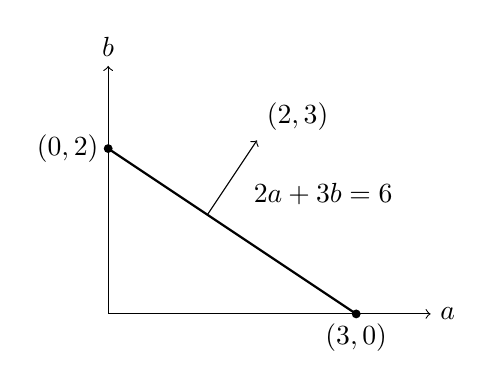
\begin{tikzpicture}[x=1.05cm,y=1.05cm]
\draw[->] (0,0)--(3.9,0) node[right]{\(a\)};
\draw[->] (0,0)--(0,3.0) node[above]{\(b\)};
\draw[thick] (0,2)--(3,0);
\fill (0,2) circle (1.6pt) node[left]{\((0,2)\)};
\fill (3,0) circle (1.6pt) node[below]{\((3,0)\)};
\draw[->] (1.2,1.2)--(1.8,2.1) node[above right]{\((2,3)\)};
\node at (2.6,1.45){\(2a+3b=6\)};
\end{tikzpicture}
\]
图的横、纵坐标是单项式 \(x^ay^b\) 的指数，不是曲线上的点坐标。这个权使 \(x^3\) 与 \(y^2\) 均有权六；代入 \(x=t^2,y=t^3\) 后，两项也同为 \(t^6\)，所以权与参数化联系起来。加入权大于六的项不会改变这条最低权关系；但这项观察本身并没有证明扰动后的曲线与原曲线同构，也没有替代完整的分支计算。

\subsection{形式解、收敛解与代数解}
\label{b3:subsec:D03:04}

设一个多项式方程组的系数属于 \(\mathbb C[x]\)。其解可能取值于代数幂级数环、收敛幂级数环或形式幂级数环。方程保持相同，允许取值的环不同；因而说“已经求出一个解”时，必须同时说明解属于哪个环。

\ProseParagraphBreak
方程 \(Y^2-(1+x)=0\) 的两个形式解是代数且收敛的，Weierstrass 除法或单根提升确定每个分支。相反，方程 \(Y-Z^2=0\) 允许任意形式级数 \(h(x)\) 给出解
\((Y,Z)=(h(x)^2,h(x))\)。若 \(h=\sum r!x^r\)，这个特定解不收敛，尽管方程的系数是多项式。所以“方程代数”并不推出“每个形式解代数”。

\begin{example}\label{b3:exm:formal-graph-not-analytic-equation}
取 \(h(x)\in x\mathbb C[\![x]\!]\) 为发散级数。在形式环中，理想
\(J=(y-h(x))\) 定义一个光滑形式图像，商环同构于 \(\mathbb C[\![x]\!]\)。然而 \(J\) 不能由一个在 \(y\) 方向导数非零的收敛函数生成：若存在收敛 \(g\) 生成 \(J\)，则 \(g=u(y-h(x))\)，其中 \(u\) 为形式单位，所以
\(\partial g/\partial y(0,0)=u(0,0)\ne0\)。收敛隐函数定理或一次的收敛 Weierstrass 预备定理使其唯一形式根收敛，矛盾。

\ProseParagraphBreak
这个结论针对给定坐标下的嵌入。作为抽象完备局部环，商仍然是一个幂级数环，当然有代数模型；不能把“这个形式图像不是解析图像”误写成“这个抽象环没有代数模型”。
\end{example}

在实际计算中，常只能确定解模 \((x)^N\) 的值。所有高于此阶的项都被舍去，因此一个有限截断既不能证明整个级数收敛，也不能排除高阶才出现的新关系。下一节的逼近定理保证某些方程的形式解可以在任意指定有限阶上由真正代数解替代；这个结论需要明确的环与方程假设。

% !TeX root = ../../Book3.tex
% 纲要标题：### D.4 形式纤维、卓越性与逼近
% 纲要位置：工作记录/计划纲要.md:2936

\section{形式纤维、卓越性与逼近}
\label{b3:sec:D04}

一组相容的形式近似不一定就是原环中的精确解，完备化的平坦性也不保证其各条纤维正则。本节在明确的底环假设下讨论这些差别，并区分有限阶逼近与实际收敛。

% 纲要内容（仅作写作计划，尚非教材正文）：
% * 完备化映射的形式纤维与卓越性的用途
% * 卓越性的来源与稳定性采用准确引用；Artin逼近限定域上有限型局部代数的Hensel化，保留Jacobian修正的可核验末步
% * 逼近意味着模高次极大理想的一致，不是任意形式解本身收敛或代数化
% * 与附录 C 的奇点理论结合阅读，不把全部消解理论作为代数学共同基础
% #### D.4.1 完备化的形式纤维与卓越性
% #### D.4.2 Artin 逼近：域上有限型情形
% #### D.4.3 有限阶逼近、收敛性与代数化
% #### D.4.4 奇点与消解理论导读


\subsection{完备化的形式纤维与卓越性}
\label{b3:subsec:D04:01}

忠实平坦性保证完备化能够检测理想与有限生成模的关系，但并不说明它的每条纤维都正则。后一个问题涉及完备化在不同素点上新增加的元素。只检查闭点的剩余域，不能回答这个问题。

\begin{definition}\label{b3:def:formal-fiber}
设 \((A,\mathfrak m)\) 为 Noether 局部环，\(\widehat A\) 为其 \(\mathfrak m\)-进完备化。对 \(\mathfrak p\in\operatorname{Spec}A\)，环
\[
\widehat A\otimes_A\kappa(\mathfrak p)
\]
称为 \(A\to\widehat A\) 在 \(\mathfrak p\) 处的\term[formalfiber]{形式纤维}[formal fiber]，其中
\(\kappa(\mathfrak p)=\operatorname{Frac}(A/\mathfrak p)\) 是该素点的剩余域。
\end{definition}

闭点处的形式纤维总是
\(\widehat A/\mathfrak m\widehat A\simeq A/\mathfrak m\)；其他素点的形式纤维不能由这一个域代替。例如
\(A=k[x]_{(x)}\) 在零素理想处的形式纤维为 \(k((x))\)，这是 \(k(x)\)-代数；附录 C 的\secref{b3:sec:C01}逐项计算了这两条纤维。若 \(A\) 本身已完备，则完备化映射为恒等，每条形式纤维才都只是相应的 \(\kappa(\mathfrak p)\)。

\begin{definition}\label{b3:def:excellent-ring}
设 \(A\) 为交换 Noether 环。
\begin{enumerate}
\item 若对每对素理想 \(\mathfrak p\subseteq\mathfrak q\)，连接二者的饱和素理想链都有相同长度，则称 \(A\) 为悬链环；饱和表示相邻两项之间不能再插入素理想。若每个有限型 \(A\)-代数都为悬链环，则称 \(A\) 具有普适链性质。
\item 设 \(F\) 为域。一个 Noether \(F\)-代数 \(B\)，若对每个有限域扩张 \(F'/F\)，环 \(B\otimes_FF'\) 都正则，则称 \(B\) 在 \(F\) 上几何正则。
\item 若对每个 \(\mathfrak p\in\operatorname{Spec}A\)，映射
\[
A_{\mathfrak p}\longrightarrow\widehat{A_{\mathfrak p}}
\]
的每条形式纤维在相应剩余域上都几何正则，则称 \(A\) 为 \(G\) 环。
\item 若对每个有限型 \(A\)-代数 \(B\)，集合
\(\operatorname{Reg}(B)=\{\mathfrak q:B_{\mathfrak q}\text{ 正则}\}\)
在 \(\operatorname{Spec}B\) 中开，则称 \(A\) 满足 \(J\)-2 条件。
\end{enumerate}
若 \(A\) 同时具有普适链性质、\(G\) 环性质及 \(J\)-2 条件，则称它为\term[excellentring]{卓越环}[excellent ring]。
\end{definition}

这里悬链环对应 catenary ring，只表示素链长度条件，不表示所有理想线性排序。几何正则要求允许有限的不可分域扩张，不能只检查可分扩张；一个域作为自身上的代数当然几何正则，但作为另一个底域上的代数就需要重新检查。第18章与第23章的不可分例子正说明底域不可省略。

\ProseParagraphBreak
卓越性的三个条件分别控制维数链、完备化纤维和正则点的邻域。完备局部环及域上有限型代数是主要来源；它们的卓越性与下面的稳定性质属于 Grothendieck 的卓越环理论。

\begin{theorem}\label{b3:thm:excellent-basic-classes}
完备 Noether 局部环是卓越环。若 \(A\) 卓越，则任意有限型 \(A\)-代数及其任意局部化也卓越；特别地，商环卓越。因而域上有限型代数及其局部化都是卓越环。
\end{theorem}
\begin{proofsketch}
完备 Noether 局部环的普适链性质采用松村英之的\cite[Theorem 29.4(ii), pp. 225--226]{Matsumura1989CommutativeRingTheory}。该证明先由 Cohen 结构定理把环表示为正则局部环的商，再用 Cohen--Macaulay 环的普适链定理；后一结果控制任意有限型代数中的素链长度，不能只用原环的一组参数的维数来代替。

\(G\) 环性质采用\cite[Theorem 32.3, pp. 257--258]{Matsumura1989CommutativeRingTheory}。这里需要检查每个局部化的形式纤维，而不只是恒等映射 \(A\to\widehat A=A\)。原证明先商去所考察纤维对应的素理想，化到完备局部整环，再用\cite[Theorem 29.4(iii), p. 226]{Matsumura1989CommutativeRingTheory}取完备正则局部子环 \(S\subseteq A\)，使 \(A\) 为有限 \(S\) 代数。令 \(K=\operatorname{Frac}S\)、\(L=\operatorname{Frac}A\)。经局部化、半局部完备化及直积分解，所考察的泛形式纤维是
\[
\bigl(\widehat{S_{\mathfrak q}}\otimes_{S_{\mathfrak q}}K\bigr)\otimes_KL
\]
的一个直积分量，其中 \(\mathfrak q\) 是所选素理想在 \(S\) 中的收缩。这说明为什么有限正则子环能够把问题归约到正则环的泛形式纤维。其几何正则性仍是关键步骤：正特征时须处理有限不可分扩张，原证明用相对形式光滑性及微分模的单射判据完成这一步。

完备局部环的 \(J\)-2 条件还采用半局部 Noether \(G\) 环满足 \(J\)-2 的定理；卓越性对有限型扩张、商及局部化的稳定性同样采用一般理论。松村在\cite[\S32, p. 260]{Matsumura1989CommutativeRingTheory}陈述这些结果，并指出多项式扩张保持 \(G\) 环性质的证明很深，转引其完整证明。上述形式纤维归约解释了这些定理中的一部分机制，正则点开放性和多项式扩张的比较定理则是这里所用而未展开的输入。最后，域是零维完备局部环，故域上有限型代数及其局部化的卓越性由前两项推出。
\end{proofsketch}

\subsection{Artin 逼近：域上有限型情形}
\label{b3:subsec:D04:02}

形式方程往往可以逐阶求解。若每一阶都能相容地继续，便得到完备化中的一个解；但这个解未必属于原环。逼近问题要求较少：给定一个有限阶数，能否在原环中找到一个准确满足方程的解，而且与这个形式解同余到该阶？

\begin{theorem}[Artin 逼近的代数情形]\label{b3:thm:artin-approximation-algebraic}
设 \(k\) 为域，\(R\) 为有限型 \(k\)-代数，\(\mathfrak p\subset R\) 为素理想，\(r,s\ge1\)。令 \((A,\mathfrak m)\) 为局部环 \(R_{\mathfrak p}\) 的 Hensel 化，\(\widehat A=\varprojlim_N A/\mathfrak m^N\) 为其 \(\mathfrak m\)-进完备化。
设
\[
F_1,\ldots,F_s\in A[Y_1,\ldots,Y_r],
\qquad
\widehat y\in\widehat A^{\,r},
\qquad F_i(\widehat y)=0\quad(1\le i\le s).
\]
则对每个整数 \(N\ge1\)，存在 \(y^{(N)}\in A^r\)，使
\[
F_i(y^{(N)})=0\quad(1\le i\le s),
\qquad
y^{(N)}-\widehat y\in\mathfrak m^N\widehat A^{\,r}.
\]
\end{theorem}

\begin{proofsketch}
本定理采用 Artin\cite[Theorem (1.10), p. 26]{Artin1969AlgebraicApproximation}的域上版本。原文把域的情形并入卓越 DVR 的情形，再于\cite[Section 5, pp. 42--44]{Artin1969AlgebraicApproximation}将一般 \(A\) 归约为多项式环在原点的 Hensel 化上的有限局部代数。有限展示把有限代数中的求解转成底环上的有限多项式方程组，这一步也处理原环中的零因子与幂零元。

证明的第一个主要输入是受控的光滑化归约。形式解定义同态 \(A[Y]/(F)\to\widehat A\)；原文在归约后的整环中取这个映射的关系理想，用卓越性保证的可分性取得泛光滑性，再用第4节的 N\'eron 型消解控制 DVR 参数处的行为\cite[Section 5, Lemma (5.6), pp. 44--46]{Artin1969AlgebraicApproximation}。没有关系时，任取足够近的元素即可；其余情形由此选出 \(G=(G_1,\ldots,G_h)\) 及一个 \(h\times h\) Jacobian 子式 \(\delta\)，使 \(\delta(\widehat y)\ne0\)。还须保留一个在形式解上非零的乘子 \(t\)，使 \(t\) 乘其余关系属于 \((G)\)；充分近的解保持 \(t(y)\ne0\)，于是整环中的 \(G(y)=0\) 推出全部关系\cite[Lemma (5.9), pp. 46--47]{Artin1969AlgebraicApproximation}。关系理想、可分性与光滑化的这些步骤采用原文的证明。

第二个主要输入是带整除条件的 Weierstrass 归纳\cite[Lemma (5.12), pp. 48--50]{Artin1969AlgebraicApproximation}。对 \(\delta(\widehat y)^2\) 作适当的坐标变换和 Weierstrass 预备，把未知级数分成次数有界的余式与商；余式系数满足少一个基底参数的有限多项式方程。先取 \(M\ge N\) 足够大，使同余于 \(\widehat y\) 模 \(\mathfrak m^M\) 的元素仍满足 \(t(y)\ne0\)；这样的 \(M\) 存在，因为 \(t(\widehat y)\ne0\)，而完备化是分离的。对余式方程归纳，并同时保留这一精度，得到 \(a\equiv\widehat y\pmod{\mathfrak m^M}\)，且
\[
G(a)\in\delta(a)^2\mathfrak m^M A^h.
\]
这里 \((A,\mathfrak m)\) 暂指归约后的 Hensel 局部整环，\(G\in A[Y_1,\ldots,Y_r]^h\)，其中 \(1\le h\le r\)。取得 \(\delta(a)^2\) 的整除条件是这一归纳的实质；只有误差属于很高的 \(\mathfrak m\) 次幂还不足以进行下面的修正。余式方程的构造及归纳的相容性采用所引引理。

说明最后的准确修正。对所选的 \(h\) 个未知量记 \(G\) 的 Jacobian 方阵为 \(J_G\)，\(\delta=\det J_G\)、\(J_G^{\mathrm{adj}}\) 为伴随矩阵。固定其余变量，代入
\(Y=a+\delta(a)J_G(a)^{\mathrm{adj}}U\)，其中这项修正只作用于所选 \(h\) 个坐标。由于 \(J_GJ_G^{\mathrm{adj}}=\delta I_h\)，Taylor 展开把 \(G(Y)=0\) 化为
\[
\delta(a)^2\bigl(e+U+Q(U)\bigr)=0,
\qquad e\in\mathfrak m^M A^h,
\]
其中 \(Q\in A[U_1,\ldots,U_h]^h\) 的各项关于 \(U\) 的次数至少二。对 \(e+U+Q(U)=0\)，零向量模 \(\mathfrak m\) 是简单零，Jacobian 为 \(I_h\)。由第23章的多变量 Jacobian 简单零提升\cref{b3:lem:henselian-jacobian-lifting}，取 \(I=\mathfrak m\)、初始点为零，可得 \(U\in\mathfrak mA^h\)；这也是原文所用的 Hensel 提升形式\cite[(1.9), pp. 25--26; Lemmas (5.10)--(5.11), pp. 47--48]{Artin1969AlgebraicApproximation}。又因 \(Q\) 没有常数项或一次项，可写 \(Q(U)=C(U)U\)，其中矩阵 \(C(U)\) 的各项属于 \(\mathfrak m\)。因此 \(I_h+C(U)\) 可逆，而
\[
U=-(I_h+C(U))^{-1}e\in\mathfrak m^MA^h.
\]
修正后的 \(y\) 便准确满足 \(G(y)=0\)，且 \(y\equiv\widehat y\pmod{\mathfrak m^M}\)，因而也同余到第 \(N\) 阶。所选精度保证 \(t(y)\ne0\)，故全部关系成立。最后经上述有限代数归约返回原环。这一伴随矩阵计算是原文 Lemma (5.10) 的修正机制，完整逼近定理还包含前面的光滑化与除法归纳。
\end{proofsketch}

更一般的卓越 Hensel 局部环上的 Artin 逼近还需一般的光滑化理论；上述原定理在这里采用的范围是域上有限型局部代数的 Hensel 化。

\ProseParagraphBreak
有两个量词必须保留。首先，\(y^{(N)}\) 对原方程是准确解，而非仅使误差属于 \(\mathfrak m^N\)。其次，\(N\) 改变时，允许选择不同的解；结论没有说存在一个 \(y\in A^r\) 与 \(\widehat y\) 在所有阶上同时相同。后一个要求在分离环中会直接迫使 \(y=\widehat y\)，强得多。

\begin{proposition}\label{b3:prop:linear-formal-approximation}
设 \((A,\mathfrak m)\) 为 Noether 局部环，\(\widehat A=\varprojlim_N A/\mathfrak m^N\) 为其 \(\mathfrak m\)-进完备化，
\(M\in\operatorname{Mat}_{s\times r}(A)\)、\(b\in A^s\)。若给定 \(\widehat y\in\widehat A^r\) 满足
\(M\widehat y=b\)，则对每个 \(N\ge1\)，存在准确解 \(y^{(N)}\in A^r\)，且
\(y^{(N)}-\widehat y\in\mathfrak m^N\widehat A^r\)。
\end{proposition}
\begin{proof}
取 \(a\in A^r\) 代表 \(\widehat y\) 模 \(\mathfrak m^N\) 的剩余类。令
\(L=M(\mathfrak m^NA^r)\subseteq A^s\)，这是有限生成模。完备化平坦且与有限生成模张量相容，所以
\[
L\widehat A=M(\mathfrak m^N\widehat A^r).
\]
误差 \(b-Ma=M(\widehat y-a)\) 属于这个子模，同时属于 \(A^s\)。由忠实平坦性，或有限生成模 \(A^s/L\) 到其完备化的单射性，可得 \(b-Ma\in L\)。故存在 \(c\in\mathfrak m^NA^r\)，使 \(Mc=b-Ma\)。取 \(y^{(N)}=a+c\)，便是所求准确解。
\end{proof}

线性情形只用有限生成模及完备化，不要求 Hensel 性。一般多项式方程中的变量乘积使误差不再由一个固定模映射控制；不能把以上证明直接套到非线性情形，也不能据此取消 Artin 定理对底环的假设。

\subsection{有限阶逼近、收敛性与代数化}
\label{b3:subsec:D04:03}

在 \(k[\![x]\!]\) 中，同余模 \((x)^N\) 表示前 \(N\) 个系数相同。它没有给剩余系数的大小任何限制，也没有断言一个任意形式关系能由多项式关系生成。

\begin{example}\label{b3:exm:approximation-does-not-converge}
在 \(\mathbb C[\![x]\!]\) 中取
\(h(x)=\sum_{j\ge1}j!x^j\)，令
\(\widehat y=(h^2,h)\)，则它准确满足 \(Y-Z^2=0\)。对每个 \(N\)，取多项式
\(h_N=\sum_{1\le j<N}j!x^j\)，便有准确的多项式解
\[
y^{(N)}=(h_N^2,h_N)
\equiv(h^2,h)\pmod{x^N}.
\]
这些准确解逼近一个发散形式解。不存在一个固定的收敛解与它在所有阶上相同，因为第二坐标的系数将被逐个确定为 \(j!\)。
\end{example}

代数化还需要说明保留什么结构。如果只问一个抽象完备环是否同构于某个代数局部环的完备化，形式坐标变换可以参与同构；若要求保留嵌入、指定函数、映射或标记，则必须把这些额外数据同时表示出来。\cref{b3:exm:formal-graph-not-analytic-equation}中的发散图像，恰好说明抽象环与指定嵌入可以有不同答案。

\ProseParagraphBreak
因此，有限阶数据最适合用来回答一个已经证明由有限阶决定的问题。例如已知一个商被 \((x)^N\) 零化时，该商的全部长度可由有限截断求出，见附录 F 的\secref{b3:sec:F04}；没有这个零化条件时，截断长度只是一个阶段性的量。有限决定性还需要额外的定理。

\subsection{奇点与消解理论导读}
\label{b3:subsec:D04:04}

结构定理使一个局部环成为正则环境中的方程商；标准基帮助计算其初始关系；形式纤维和逼近则比较不同局部对象。这些方法都能用于奇点，但它们本身不等于一个一般奇点消解定理。

\ProseParagraphBreak
最简单的平面曲线已经显示为什么要更换环境。对尖点
\(y^2=x^3\)，在原点外取新的比值坐标 \(v=y/x\)，代入 \(y=xv\) 得
\[
y^2-x^3=x^2(v^2-x).
\]
方程 \(v^2-x=0\) 定义光滑曲线，以 \(v\) 为参数，原坐标变成
\[
x=v^2,\qquad y=v^3.
\]
这与正规化的参数完全一致。保留全部乘积方程会额外留下由 \(x^2\) 定义的部分；取原点外曲线在新坐标图中的闭包，才得到严格变换 \(v^2-x=0\)。代数上，这是把总变换理想对 \(x\) 作饱和后收缩。

\ProseParagraphBreak
这一个坐标图是原点吹起的常见图。另一图取 \(x=yw\)，约去总变换中的 \(y^2\) 后得到 \(1-yw^3=0\)，在 \(y=0\) 上没有点，所以它不会增加尖点上方的新分支。两个图的相容关系解释了比值坐标如何合起来；若要把它作为一般几何构造，还须建立图的粘合、射影性及固有性等性质。

\ProseParagraphBreak
对于更高维对象，正规化通常不能消除全部奇点，局部图中的参数计算也不足以保证一种操作能在有限步后结束。一般消解理论要控制所选中心、例外部分和维数递降，并对特征及几何对象作准确限制。它所解决的是把奇异空间改造成正则空间的问题；自由消解则是在同一个底环上用自由模和正合复形描述模。二者都可参与奇点研究，却是不同的构造。


\begin{chaptersummary}
有限阶商可以相同，环本身仍可能不同。Hensel 化使单根与互素因式能够提升，完备化补入所有相容极限，解析环则另外要求系数有实际收敛范围。比较它们必须给出底环、局部同态及所用拓扑。

\ProseParagraphBreak
Cohen 结构定理中，系数对象的存在是深层步骤；选定它以后，极大理想的有限生成性与完备性给出逐阶展开。等特征采用系数域，混合特征采用保留 \(p\) 的 Cohen 环。得到正则局部覆盖，并没有自动得到正则序列关系。

\ProseParagraphBreak
形式 Weierstrass 除法通过提高误差的系数理想阶数来收敛；解析除法另外用绝对系数范数控制收缩算子，保证所得商与余式实际收敛。曲线算例进一步表明：一个分支可以有重切线，有限映射的秩可以大于一般点以外的不同点数，交数则由有限长度商保留接触信息。

\ProseParagraphBreak
卓越性控制素链、形式纤维和正则点的开性。Artin 逼近在指定环类中把形式解的有限阶信息实现为准确解，但不保证原来的形式解收敛，也不自动建立带全部附加结构的代数化。一般奇点消解仍需独立的几何理论。
\end{chaptersummary}

\BookExercises

\begin{exercise}\label{b3:ex:D-local-units-truncations}
证明 \(\mathbb C\{x_1,\ldots,x_n\}\) 的单位恰为常数项非零的级数，并证明它模 \((x)^N\) 的商与多项式环的同阶商相同。
\end{exercise}
\begin{solution}
常数项非零时，级数在一个较小多圆盘上不为零，倒数由局部几何级数展开得到，仍收敛；常数项为零时不能与任何级数相乘得到常数项 \(1\)。任意收敛级数减去次数小于 \(N\) 的 Taylor 多项式后，只剩次数至少 \(N\) 的项。把这些项按一个次数 \(N\) 的单项式因子分成有限组，每组除去该单项式后仍在较小多圆盘绝对收敛，故余项属于 \((x)^N\)。于是每个剩余类均有有限多项式代表，核也恰为次数至少 \(N\) 的多项式理想。
\end{solution}

\begin{optionalexercise}\label{b3:ex:D-hensel-not-rational}
求满足 \(u^2=1+x,\ u(0)=1\) 的级数到 \(x^3\) 项，并证明它属于 \((\mathbb Q[x]_{(x)})^{\mathrm h}\)，却不属于 \(\mathbb Q(x)\)。
\end{optionalexercise}
\begin{solution}
比较系数得到
\[
u=1+\frac12x-\frac18x^2+\frac1{16}x^3+O(x^4).
\]
剩余根 \(1\) 处导数为 \(2\)，在 \(\mathbb Q\) 中可逆，因此 Hensel 化中存在唯一该分支。若它是有理函数，则 \(1+x\) 为有理函数的平方；平方在每个素因子处的阶数为偶数，而 \(x+1\) 的阶数为一，矛盾。
\end{solution}

\begin{exercise}\label{b3:ex:D-coefficient-field-nonunique}
令 \(K=\mathbb Q(t)\)、\(B=K[\varepsilon]/(\varepsilon^2)\)，\(\pi:B\to K\) 为商映射。分类所有满足 \(\pi\sigma=\operatorname{id}_K\) 的 \(\mathbb Q\) 代数同态 \(\sigma:K\to B\)，并证明它们的像都是系数域。说明两个截面不同是否可能有相同的像。
\end{exercise}
\begin{solution}
每个截面唯一由 \(\sigma(t)=t+c\varepsilon\)、\(c\in K\) 决定。对有理函数 \(r(t)\)，其值必须为
\[
\sigma_c(r)=r+c\,r'\varepsilon.
\]
乘法的 Leibniz 公式与 \(\varepsilon^2=0\) 保证这确为 \(\mathbb Q\) 代数同态；对非零有理函数 \(r\)，\(\sigma_c(r)\) 的 \(\varepsilon^0\) 系数就是 \(r\ne0\)，所以分母的像可逆。它与 \(\pi\) 的复合为恒等，故单射，其像经剩余域映射同构于 \(K\)，就是系数域。若两个像相同，\(\pi\) 在该子域上的逆唯一，两截面必相同；因此不同 \(c\) 给出不同系数子域。
\end{solution}

\begin{exercise}\label{b3:ex:D-minimal-cohen-kernel}
设 \(k\) 为域，\(A=k[\![u,v]\!]/(u^2,v^2)\)。给出连续满射
\(k[\![U,V,W]\!]\to A\)，令 \(U,V,W\) 分别映到 \(\bar u,\bar v,\bar u+\bar v\)。求其核、\(\dim A\)、嵌入维数及长度，构造一个极小 Cohen 表示，并解释变量个数与 Krull 维数为何不同。
\end{exercise}
\begin{solution}
连续换元 \(W'=W-U-V\) 将映射变为 \(W'\mapsto0\)，其核恰为 \((W-U-V,U^2,V^2)\)。商有 \(k\) 基 \(1,\bar u,\bar v,\bar u\bar v\)，极大理想幂零，故维数为零、长度为四。\(\mathfrak m/\mathfrak m^2\) 以 \(\bar u,\bar v\) 为基，所以嵌入维数为二。极小表示就是 \(k[\![U,V]\!]/(U^2,V^2)\)，其核落在 \((U,V)^2\) 内。三变量表示中有可线性消去的 \(W-U-V\)；极小变量数读的是嵌入维数，不能用 Krull 维数零代替。
\end{solution}

\begin{exercise}\label{b3:ex:D-characteristic-obstruction}
证明 \(\mathbb Z_p\) 与 \(\mathbb Z/p^2\mathbb Z\) 都不可能是 \(\mathbb F_p[\![X_1,\ldots,X_n]\!]\) 的保单位商环。说明二者可使用的系数对象有何不同。
\end{exercise}
\begin{solution}
\(\mathbb F_p[\![X]\!]\) 的任何非零保单位商满足 \(p\cdot1=0\)，而所给两环中这个元素均非零，所以都不可能。第一环本身是 Cohen 环，特征为零；第二环可由 Cohen 环 \(\mathbb Z_p\) 商去 \(p^2\) 得到，其系数子环为 \(\mathbb Z/p^2\mathbb Z\)，有非零幂零元 \(p\)，不是 DVR。
\end{solution}

\begin{exercise}\label{b3:ex:D-ramified-model}
设 \(C=\mathbb Z_p\)、\(A=C[\![T]\!]/(T^3-p)\)。证明 \(A\) 为 DVR，作为 \(C\)-模自由秩为 \(3\)，且 \(v_A(p)=3\)。
\end{exercise}
\begin{solution}
形式 Weierstrass 除法给出基 \(1,\bar T,\bar T^2\)，所以 \(C\) 注入 \(A\)，且模秩为 \(3\)。环境环 \(C[\![T]\!]\) 是二维正则局部整环，商去非零非单位 \(T^3-p\) 后维数为一。商的极大理想由 \(\bar T\) 生成，因此它正则，并由一维正则局部环的刻画为 DVR。以 \(\bar T\) 为统一化元，归一化离散赋值满足 \(v_A(\bar T)=1\)，故等式 \(p=\bar T^3\) 给出 \(v_A(p)=3\)。
\end{solution}

\begin{exercise}\label{b3:ex:D-artinian-ci-models}
求 \(A=k[\![u,v]\!]/(u^2,v^3)\) 和 \(B=k[\![u,v]\!]/(u,v)^2\) 的长度及基座维数，并据此判断它们是否为完全交。
\end{exercise}
\begin{solution}
\(A\) 有基 \(1,u,v,uv,v^2,uv^2\)，长度为 \(6\)。同时被 \(u,v\) 零化的元素恰为 \(k\,uv^2\)，所以基座一维。关系 \(u^2,v^3\) 是正则序列，故 \(A\) 为完全交。\(B\) 有基 \(1,u,v\)，长度为 \(3\)，基座为 \(ku+kv\)，二维，因此由零维完全交的基座判据知 \(B\) 不是完全交。基座一维本身在本题并不被用作充分条件；\(A\) 的正面判断来自明确正则序列。
\end{solution}

\begin{exercise}\label{b3:ex:D-explicit-series-division}
在 \(k[\![x]\!][\![T]\!]\) 中，把 \(h=(1-T)^{-1}\) 除以 \(f=T^2-x\)，准确求出商和余式。
\end{exercise}
\begin{solution}
因为
\[
\frac1{1-T}-\frac{1+T}{1-x}
=\frac{T^2-x}{(1-T)(1-x)},
\]
所以商为 \(((1-T)(1-x))^{-1}\)，余式为
\((1-x)^{-1}+T(1-x)^{-1}\)。两个分母常数项均为 \(1\)，其倒数在所给形式环中存在。余式关于 \(T\) 的次数小于二；除法唯一性说明这就是唯一答案。
\end{solution}

\begin{exercise}\label{b3:ex:D-weierstrass-hypothesis}
令 \(A=k[\![x]\!]\)、\(B=A[\![T]\!]/(T^2+xT+x^3)\)，其中 \(k\) 为域。证明 \(B\) 在 \(A\) 上自由，求乘 \(\bar T\) 的矩阵，并把 \((1-\bar T)^{-1}\) 写成唯一的一次余式。核验这个余式与形式几何级数 \(\sum_{j\ge0}\bar T^j\) 相同。
\end{exercise}
\begin{solution}
模 \((x)\) 的多项式为 \(T^2\)，所以 Weierstrass 除法给出基 \(1,\bar T\)。乘法矩阵为
\[
\begin{pmatrix}0&-x^3\\1&-x\end{pmatrix}.
\]
因为 \(1+x+x^3\) 在 \(A\) 中可逆，且
\[
(1-\bar T)(1+x+\bar T)=1+x+x^3,
\]
逆元的余式为 \((1+x+\bar T)/(1+x+x^3)\)。\(B\) 是完备局部环，\(\bar T\) 属于极大理想，因此几何级数收敛并乘 \(1-\bar T\) 得一；逆元唯一，故等于该余式。
\end{solution}

\begin{exercise}\label{b3:ex:D-finite-multiplication-matrix}
设 \(A=k[\![x]\!]\)、\(B=A[\![T]\!]/(T^3+xT+x)\)。写出乘以 \(\bar T\) 关于基 \(1,\bar T,\bar T^2\) 的矩阵，求该算子的迹、行列式和特征多项式。
\end{exercise}
\begin{solution}
由 \(\bar T^3=-x-x\bar T\)，矩阵为
\[
\begin{pmatrix}
0&0&-x\\
1&0&-x\\
0&1&0
\end{pmatrix}.
\]
迹为 \(0\)，行列式为 \(-x\)，直接计算 \(\det(\lambda I-M)\) 得
\(\lambda^3+x\lambda+x\)。Weierstrass 除法保证所用三个元素确实是模基，因此这些矩阵量属于给定有限自由代数的准确计算。
\end{solution}

\begin{exercise}\label{b3:ex:D-cusp-conductor}
设 \(A=k[\![t^2,t^3]\!]\subseteq C=k[\![t]\!]\)。求 \(C/A\) 的 \(k\)-维数与导子
\(\mathfrak c=\{c\in C:cC\subseteq A\}\)，并把导子写成 \(A\) 的理想。
\end{exercise}
\begin{solution}
\(A=k+t^2k[\![t]\!]\)，只缺少一次项，所以 \(C/A\) 由 \(t\) 的剩余类张成，维数为 \(1\)。若 \(cC\subseteq A\)，先由 \(c\in A\) 知它没有一次项；再由 \(ct\in A\) 知它的常数项为零，故 \(c\in t^2C\)。反过来 \(t^2C\subseteq A\)，且它是 \(C\)-理想，当然满足要求。因此导子为 \(t^2C=(t^2,t^3)A\)。
\end{solution}

\begin{exercise}\label{b3:ex:D-node-completion-branches}
令 \(u=\sqrt{1+x}\in\mathbb C[\![x]\!]\)、\(u(0)=1\)，取
\(B=\mathbb C[\![x,y]\!]/(y^2-x^2(1+x))\)。用两分支求值将 \(B\) 嵌入 \(C=\mathbb C[\![x]\!]\times\mathbb C[\![x]\!]\)，求像、正规化与导子理想 \(\{c\in C:cC\subseteq B\}\)，并计算 \(C/B\) 的长度。
\end{exercise}
\begin{solution}
Weierstrass 除法使每个元素唯一写成 \(a(x)+b(x)y\)，两分支值为 \((a+bxu,a-bxu)\)，故求值映射单射。像恰为常数项相等的级数对：反向取 \(a=(r+s)/2\)、\(b=(r-s)/(2xu)\)，后式因常数项相等而属于 \(\mathbb C[\![x]\!]\)。所以差常数项映射给出正合列
\[
0\longrightarrow B\longrightarrow C\longrightarrow\mathbb C\longrightarrow0.
\]
环 \(C=B+B(1,0)\) 有限于 \(B\)，幂等元 \((1,0)\) 整，且在两分支的全分式环中 \(C\) 为两个 DVR 的乘积，整闭。任意全分式环中对 \(B\) 整的元素也对 \(C\) 整，必已属于整闭环 \(C\)。反向的整性由上述有限性保证，故 \(C\) 恰为 \(B\) 的正规化。要使 \((r,s)C\) 的任意乘积都具有相同常数项，必须且只须 \(r(0)=s(0)=0\)，所以导子为 \(xC\)，它在 \(B\) 中对应极大理想 \((x,y)\)。上述正合列又给出 \(C/B\) 长度为一。
\end{solution}

\begin{exercise}\label{b3:ex:D-cusp-contacts}
令 \(f=y^2-x^3\)。对每个整数 \(m\ge2\)，计算
\(i_0(f,y-x^m)\)，并与 \(i_0(f,y-\lambda x)\)、\(\lambda\ne0\)，比较。
\end{exercise}
\begin{solution}
商去 \(y-x^m\) 后，方程成为
\(x^{2m}-x^3=x^3(x^{2m-3}-1)\)。括号内常数项为 \(-1\)，是单位，故商为 \(\mathbb C[\![x]\!]/(x^3)\)，交数为 \(3\)。非切线 \(y-\lambda x\) 给出交数 \(2\)。这些结果表示高阶曲线 \(y=x^m\) 与切线 \(y=0\) 都在尖点具有三阶接触；次数更大的 \(m\) 不使本例的交数继续增大。
\end{solution}

\begin{exercise}\label{b3:ex:D-newton-weight}
对 \(f=y^2-x^3+x^2y^2+y^5\) 取权 \(w(x)=2,w(y)=3\)。求最低权部分，写出 Newton 多边形的有界边，并说明哪些关于分支的结论尚不能仅由这个计算得出。
\end{exercise}
\begin{solution}
四项的权分别为 \(6,6,10,15\)，所以最低权部分为 \(y^2-x^3\)。指数 \((2,2),(0,5)\) 都位于由 \((3,0),(0,2)\) 加正象限所得凸集内，因此有界边仍是连接 \((3,0)\) 与 \((0,2)\) 的线段。这个结果确定初始关系与候选权，但没有独立证明完整方程的不可约性、分支参数化或与标准尖点的解析同构；这些都需要进一步除法或坐标变换。
\end{solution}

\begin{exercise}\label{b3:ex:D-formal-fiber-closed}
设 \((A,\mathfrak m,k)\) 为 Noether 局部环。证明其闭点形式纤维为 \(k\)。若 \(A\) 已完备，求每个素点的形式纤维，并解释为什么后一结论不能仅由闭点结论推出。
\end{exercise}
\begin{solution}
\(\widehat A\otimes_Ak=\widehat A/\mathfrak m\widehat A\simeq A/\mathfrak m=k\)。若 \(A=\widehat A\)，则
\(\widehat A\otimes_A\kappa(\mathfrak p)=\kappa(\mathfrak p)\) 对所有素点成立。闭点等式对每个 Noether 局部环都成立，并不能推出 \(A\to\widehat A\) 为同构；例如 \(k[x]_{(x)}\) 的泛点形式纤维为 \(k(\!(x)\!)\)，它不等于原泛点域 \(k(x)\)。
\end{solution}

\begin{exercise}\label{b3:ex:D-excellence-conditions}
设 \(k\) 为域，\(A=k[\![x,y]\!]\)，\(\mathfrak p=(x)A\)。分别写出检验 \(A\) 的 G 环、J-2 和普适链性质需要考察的对象，并说明等式 \(A=\widehat A\) 自动计算了哪些形式纤维。证明 \(A_{\mathfrak p}\) 的剩余域为 \(k(\!(y)\!)\)，解释原环的完备性为什么不能直接取代这个局部环的形式纤维验证。
\end{exercise}
\begin{solution}
G 环条件要求对每个 \(\mathfrak q\in\operatorname{Spec}A\)，局部完备化映射 \(A_{\mathfrak q}\to\widehat{A_{\mathfrak q}}\) 平坦且每条纤维几何正则。J-2 要求每个有限型 \(A\) 代数的正则点集为开集；普适链性质则要求这些有限型代数中具有相同端点的饱和素链长度一致。后两个条件涉及新的有限型代数，均不是对某一个完备化映射的计算。

由 \(A=\widehat A\)，只能立即得到这个映射在任意 \(\mathfrak q\) 处的纤维为 \(\kappa(\mathfrak q)\)。对于 G 环，所需映射却是各个 \(A_{\mathfrak q}\) 到其自身完备化的映射。在指定点 \(\mathfrak p\) 处，\(A/\mathfrak p=k[\![y]\!]\)，故
\[
\kappa(\mathfrak p)=\operatorname{Frac}(A/\mathfrak p)=k(\!(y)\!).
\]
这里的局部环 \(A_{\mathfrak p}\) 采用 \(\mathfrak pA_{\mathfrak p}\)-进拓扑，而原环完备性采用 \((x,y)\)-进拓扑；局部化倒置了所有不在 \(\mathfrak p\) 中的元素，不能把两种完备化当作同一个环。完备 Noether 局部环确实是 G 环，但该结论还需要\cref{b3:thm:excellent-basic-classes}所引用的一般定理。
\end{solution}

\begin{exercise}\label{b3:ex:D-linear-approximation}
设 \(A=k[x]_{(x)}\)，在 \(k[\![x]\!]\) 中给定解
\[
(1-x)Y+xZ=1,\qquad Z=h(x),
\]
其中 \(h(x)\) 为任意形式级数。对每个 \(N\)，构造 \(A\) 中的准确解，与给定解同余模 \(x^N\)。
\end{exercise}
\begin{solution}
取 \(h_N\in k[x]\) 为 \(h\) 模 \(x^N\) 的截断，令
\[
Z_N=h_N,\qquad Y_N=\frac{1-xh_N}{1-x}\in A.
\]
它们准确满足方程。给定解的第一坐标为
\((1-xh)/(1-x)\)，故第一坐标之差属于 \(x^{N+1}k[\![x]\!]\)，第二坐标之差属于 \(x^Nk[\![x]\!]\)。所求同余成立；此构造不要求 \(h\) 收敛或代数。
\end{solution}

\begin{exercise}\label{b3:ex:D-artin-quantifiers}
对方程 \(Y-Z^2=0\) 与形式解
\(\widehat y=(h^2,h)\)，其中 \(h=\sum_{j\ge1}j!x^j\)，证明存在任意阶的准确多项式近似，却不存在一个准确收敛解与 \(\widehat y\) 在所有阶上相同。指出这与 Artin 逼近的量词是否冲突。
\end{exercise}
\begin{solution}
取 \(h_N\) 为次数小于 \(N\) 的截断，则 \((h_N^2,h_N)\) 为准确多项式解，并与 \(\widehat y\) 同余模 \(x^N\)。若同一个收敛解对每个 \(N\) 都同余，则分离性使其第二坐标等于 \(h\)，与 \(h\) 发散矛盾。Artin 逼近允许解依赖 \(N\)，所以不存在冲突；把“对每个 \(N\) 存在一个解”换成“存在一个解对每个 \(N\) 都成立”，正是错误加强。
\end{solution}

\begin{exercise}\label{b3:ex:D-cusp-strict-transform}
对尖点 \(y^2=x^3\)，在坐标图 \(y=xv\) 中分别写出总变换与严格变换的理想，并证明
\((x^2(v^2-x)):x^\infty=(v^2-x)\) 在 \(\mathbb C[x,v]\) 中成立。
\end{exercise}
\begin{solution}
总变换为 \((x^2(v^2-x))\)。把 \(x\) 变成可逆元后，因子 \(x^2\) 可消去，故饱和至少包含 \((v^2-x)\)。另一方面，商
\(\mathbb C[x,v]/(v^2-x)\simeq\mathbb C[v]\) 中 \(x\) 对应 \(v^2\)，是非零因子。因此若 \(x^Ng\) 属于 \((v^2-x)\)，则 \(g\) 已属于它；这说明后者已对 \(x\) 饱和，给出反向包含。严格变换为 \(v^2-x=0\)，是以 \(v\) 为参数的光滑曲线。
\end{solution}
